
\documentclass{llncs}
\usepackage{graphicx}        % standard LaTeX graphics tool
                             % when including figure files
\usepackage{subfigure}
\usepackage{url}
%%%%%%%%%%%%%%%%%%%%%%%%%%%%%%%%%%%%%%%%%%%%%%%%%%%%%%%%%%%%%%%%%%%%%%%%%%%%%%%%%%%%%%%%%

\begin{document}
\sloppy

\title{Random Selection of Parameters in Asynchronous Pool-Based Evolutionary Algorithms}

\author{Mario Garc\'ia-Valdez\inst{1} \and Ren\'e M\'arquez\inst{1} \and Juan J. Merelo Guerv\'os\inst{2} \and  Leonardo Trujillo \inst{1}}

\institute{Instituto Tecnol\'ogico de Tijuana, Tijuana BC, Mexico
\and
Universidad de Granada, Granada, Spain
\email{mario@tectijuana.edu.mx}\\
\email{renemarquezvalenzuela@gmail.com}\\
\email{jmerelo@geneura.ugr.es}\\
\email{leonardo.trujillo@tectijuana.edu.mx}}

\maketitle

\begin{abstract}
It is not always possible to set up an distributed system with
homogeneous nodes to run algorithms in a synchronous way. In grid,
cloud or volunteer setups nodes are heterogeneous, or simply are not
available at the exact same time; this is a challenge for the researcher if
their full performance is going to be actually leveraged. We are
interested in evolutionary algorithms (EAs), which evolve a population
of solutions using a mechanism inspired by biological evolution; in this field, 
several asynchronous Evolutionary Algorithms (EAs) that distribute the
evolutionary process among heterogeneous nodes have
been proposed. These algorithms make the population shared between
distributed workers  which execute the actual evolutionary
process by taking samples of the population, and replacing them in the
population pool by evolved individuals. The performance of these EAs
depends in part on the selection of parameters for the EA running in
each worker, which may include sample size, generations, mutation rate
and crossover rate along with the overall configuration. In this paper
we present a method inspired by a strategy proposed by Gong and Fukunaga for the
Island-Model which statically assigns random parameter settings to
each island in a cloud setting. Experiments were conducted in the
cloud using 2, 6 and 12 virtual machine configurations, with
both homogeneous and heterogeneous random settings using five 
test functions for single-objective optimization (Rastrigin, Griewank, De Jong, Schaffer 
and Ackley) and the OneMax binary problem. The results suggest that this approach can yield
performance improvements which are competitive with instances of the
algorithm using workers with control parameters tuned specifically for
the benchmark.

\keywords{Distributed Evolutionary Algorithms, Volunteer Computing,
  Cloud Computing}
\end{abstract}
\section{Introduction}
% EA Paramaters 
% Worst on many workers
% Explore and Exploit
% Dynamic adaptation
% Random Patameters
% Evaluate in EvoSpace

\section{Related Work}
% Dynamic adaptation
% Random Patameters

\section{EvoSpace Cloud Implementation}
% Architecture Components
% Random Patameters


\section{Experiments}

\section{Set up}


\begin{figure*}[t]
    \centering
        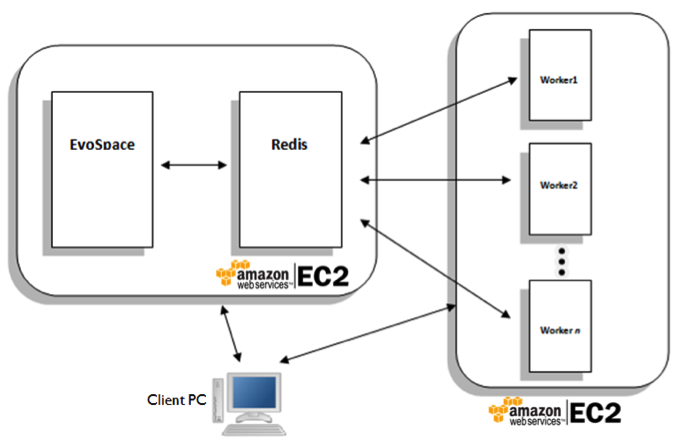
\includegraphics[width=10cm]{img/evospace-aws.png}
    \caption{Main components and data-flow in the cloud version of EvoSpace. }
    \label{fig:evospace}
\end{figure*}

\subsection{One Max}

\begin{figure*}[b]
    \centering
    \subfigure [2 workers]
    {
        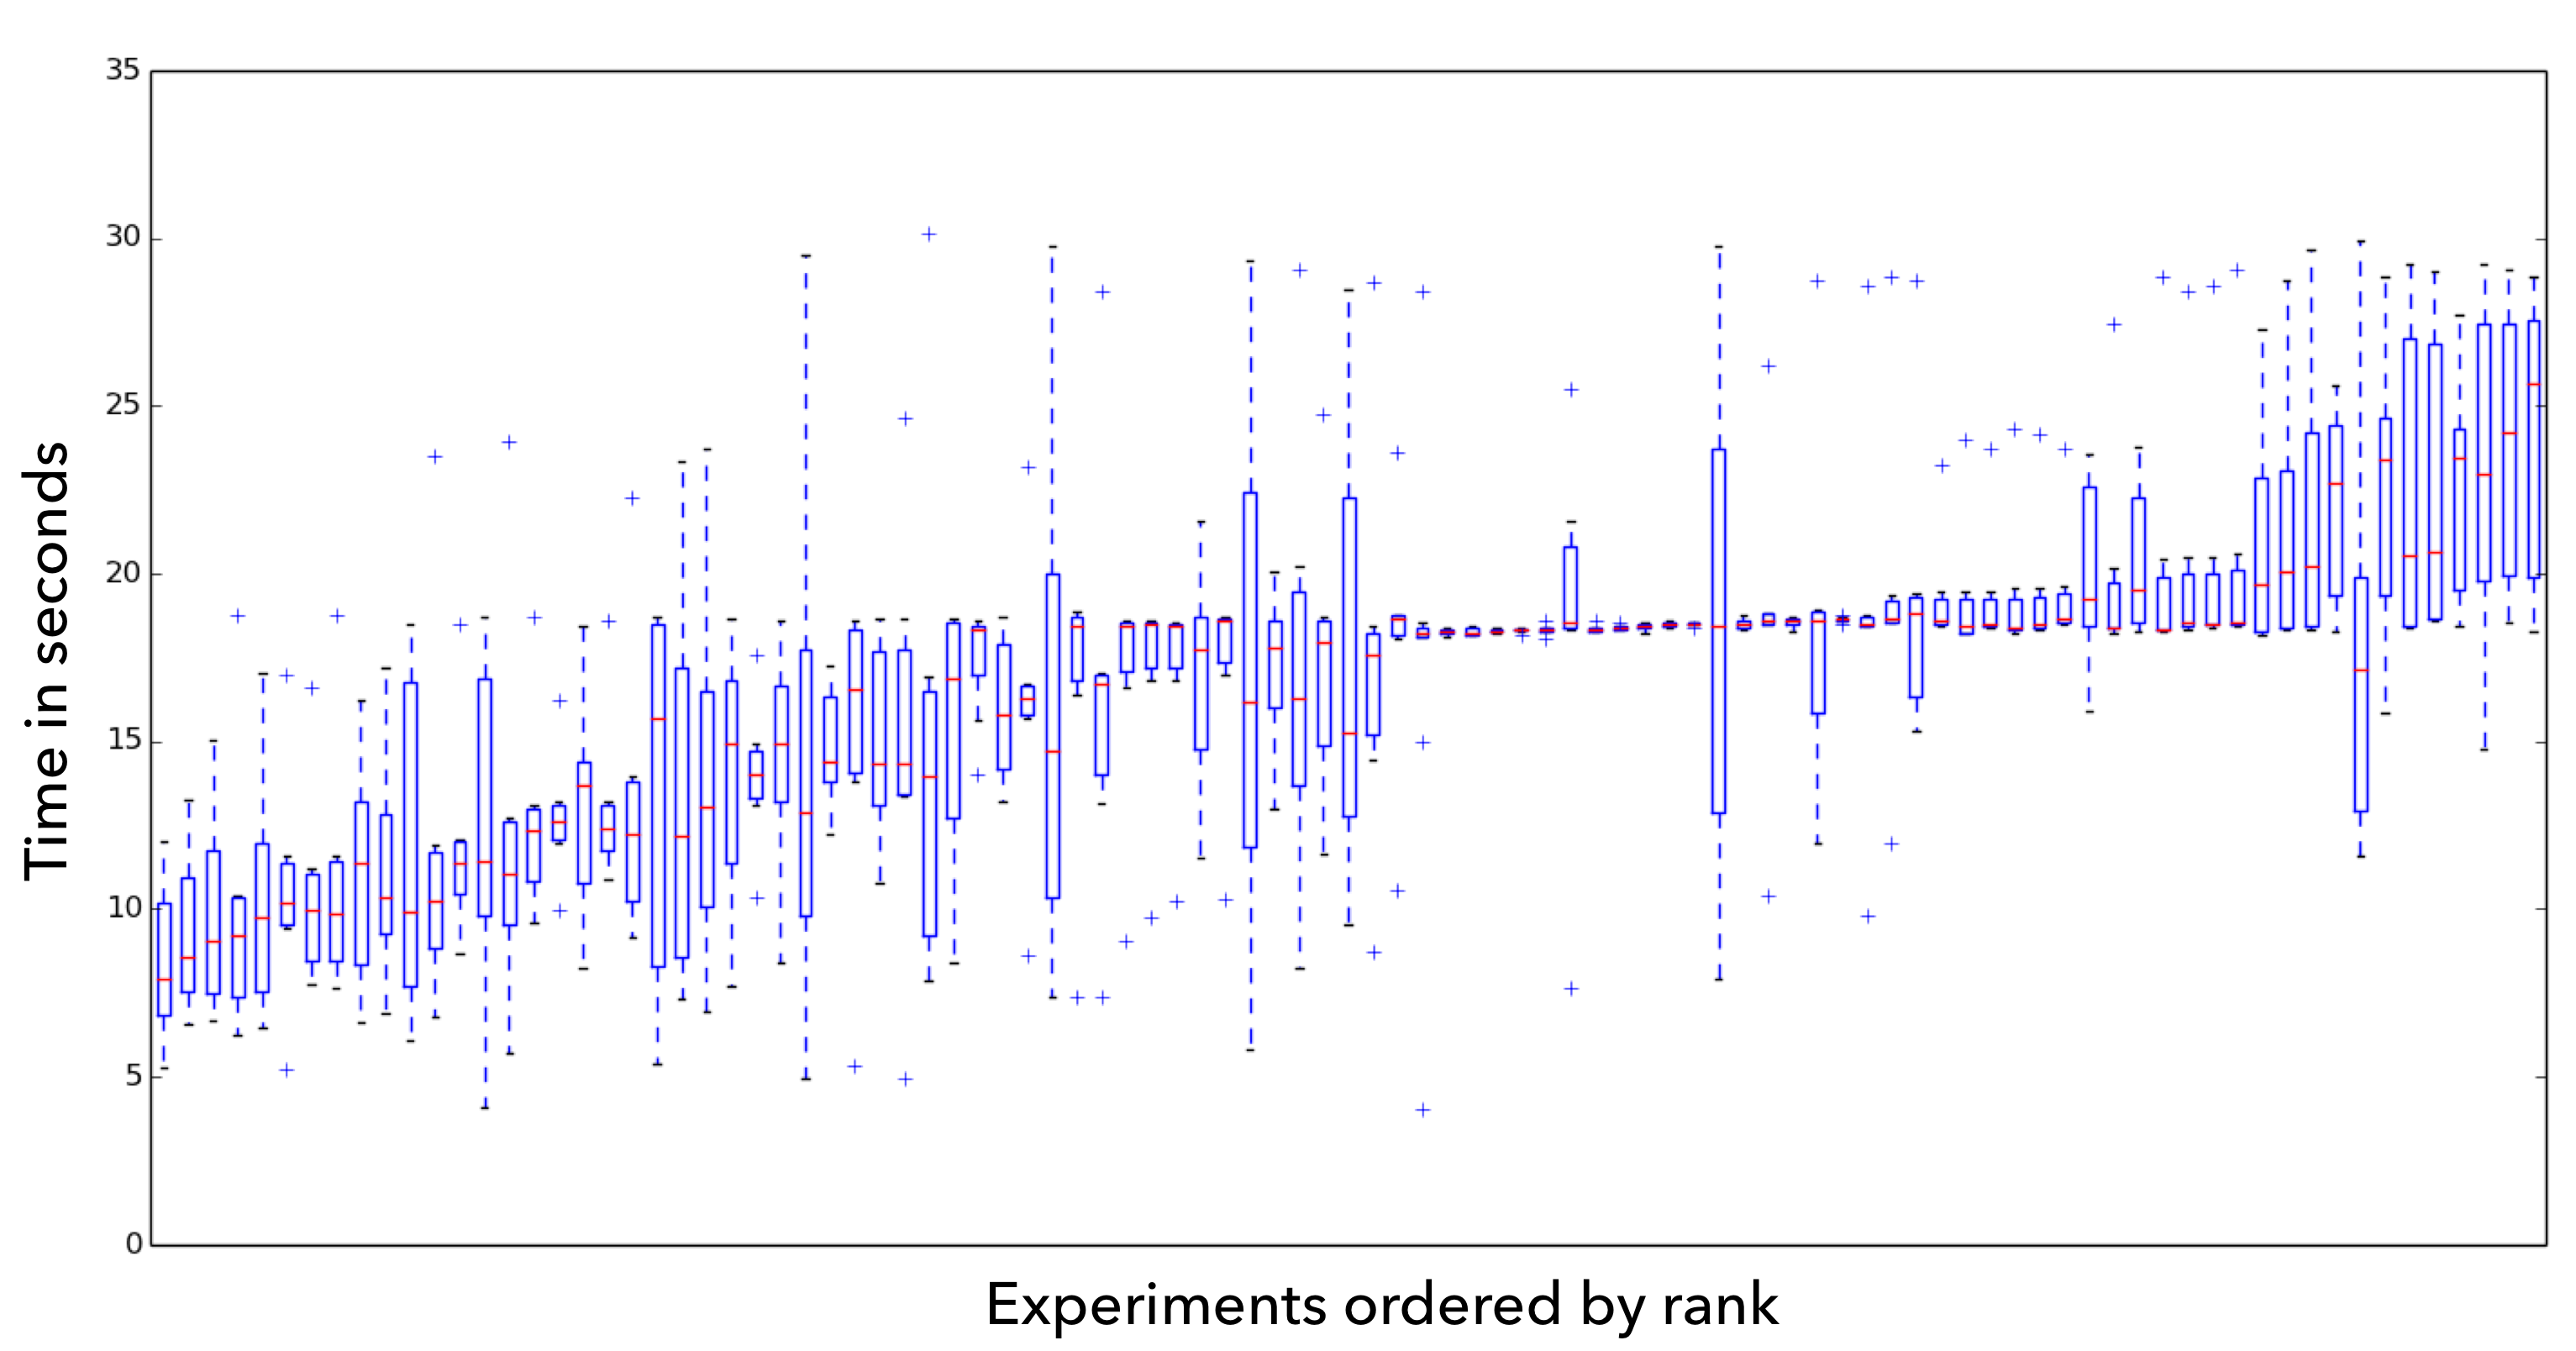
\includegraphics[width=3in]{img/2w_onemax_100_box.png}
    }
    \subfigure  [6 workers]
    {
        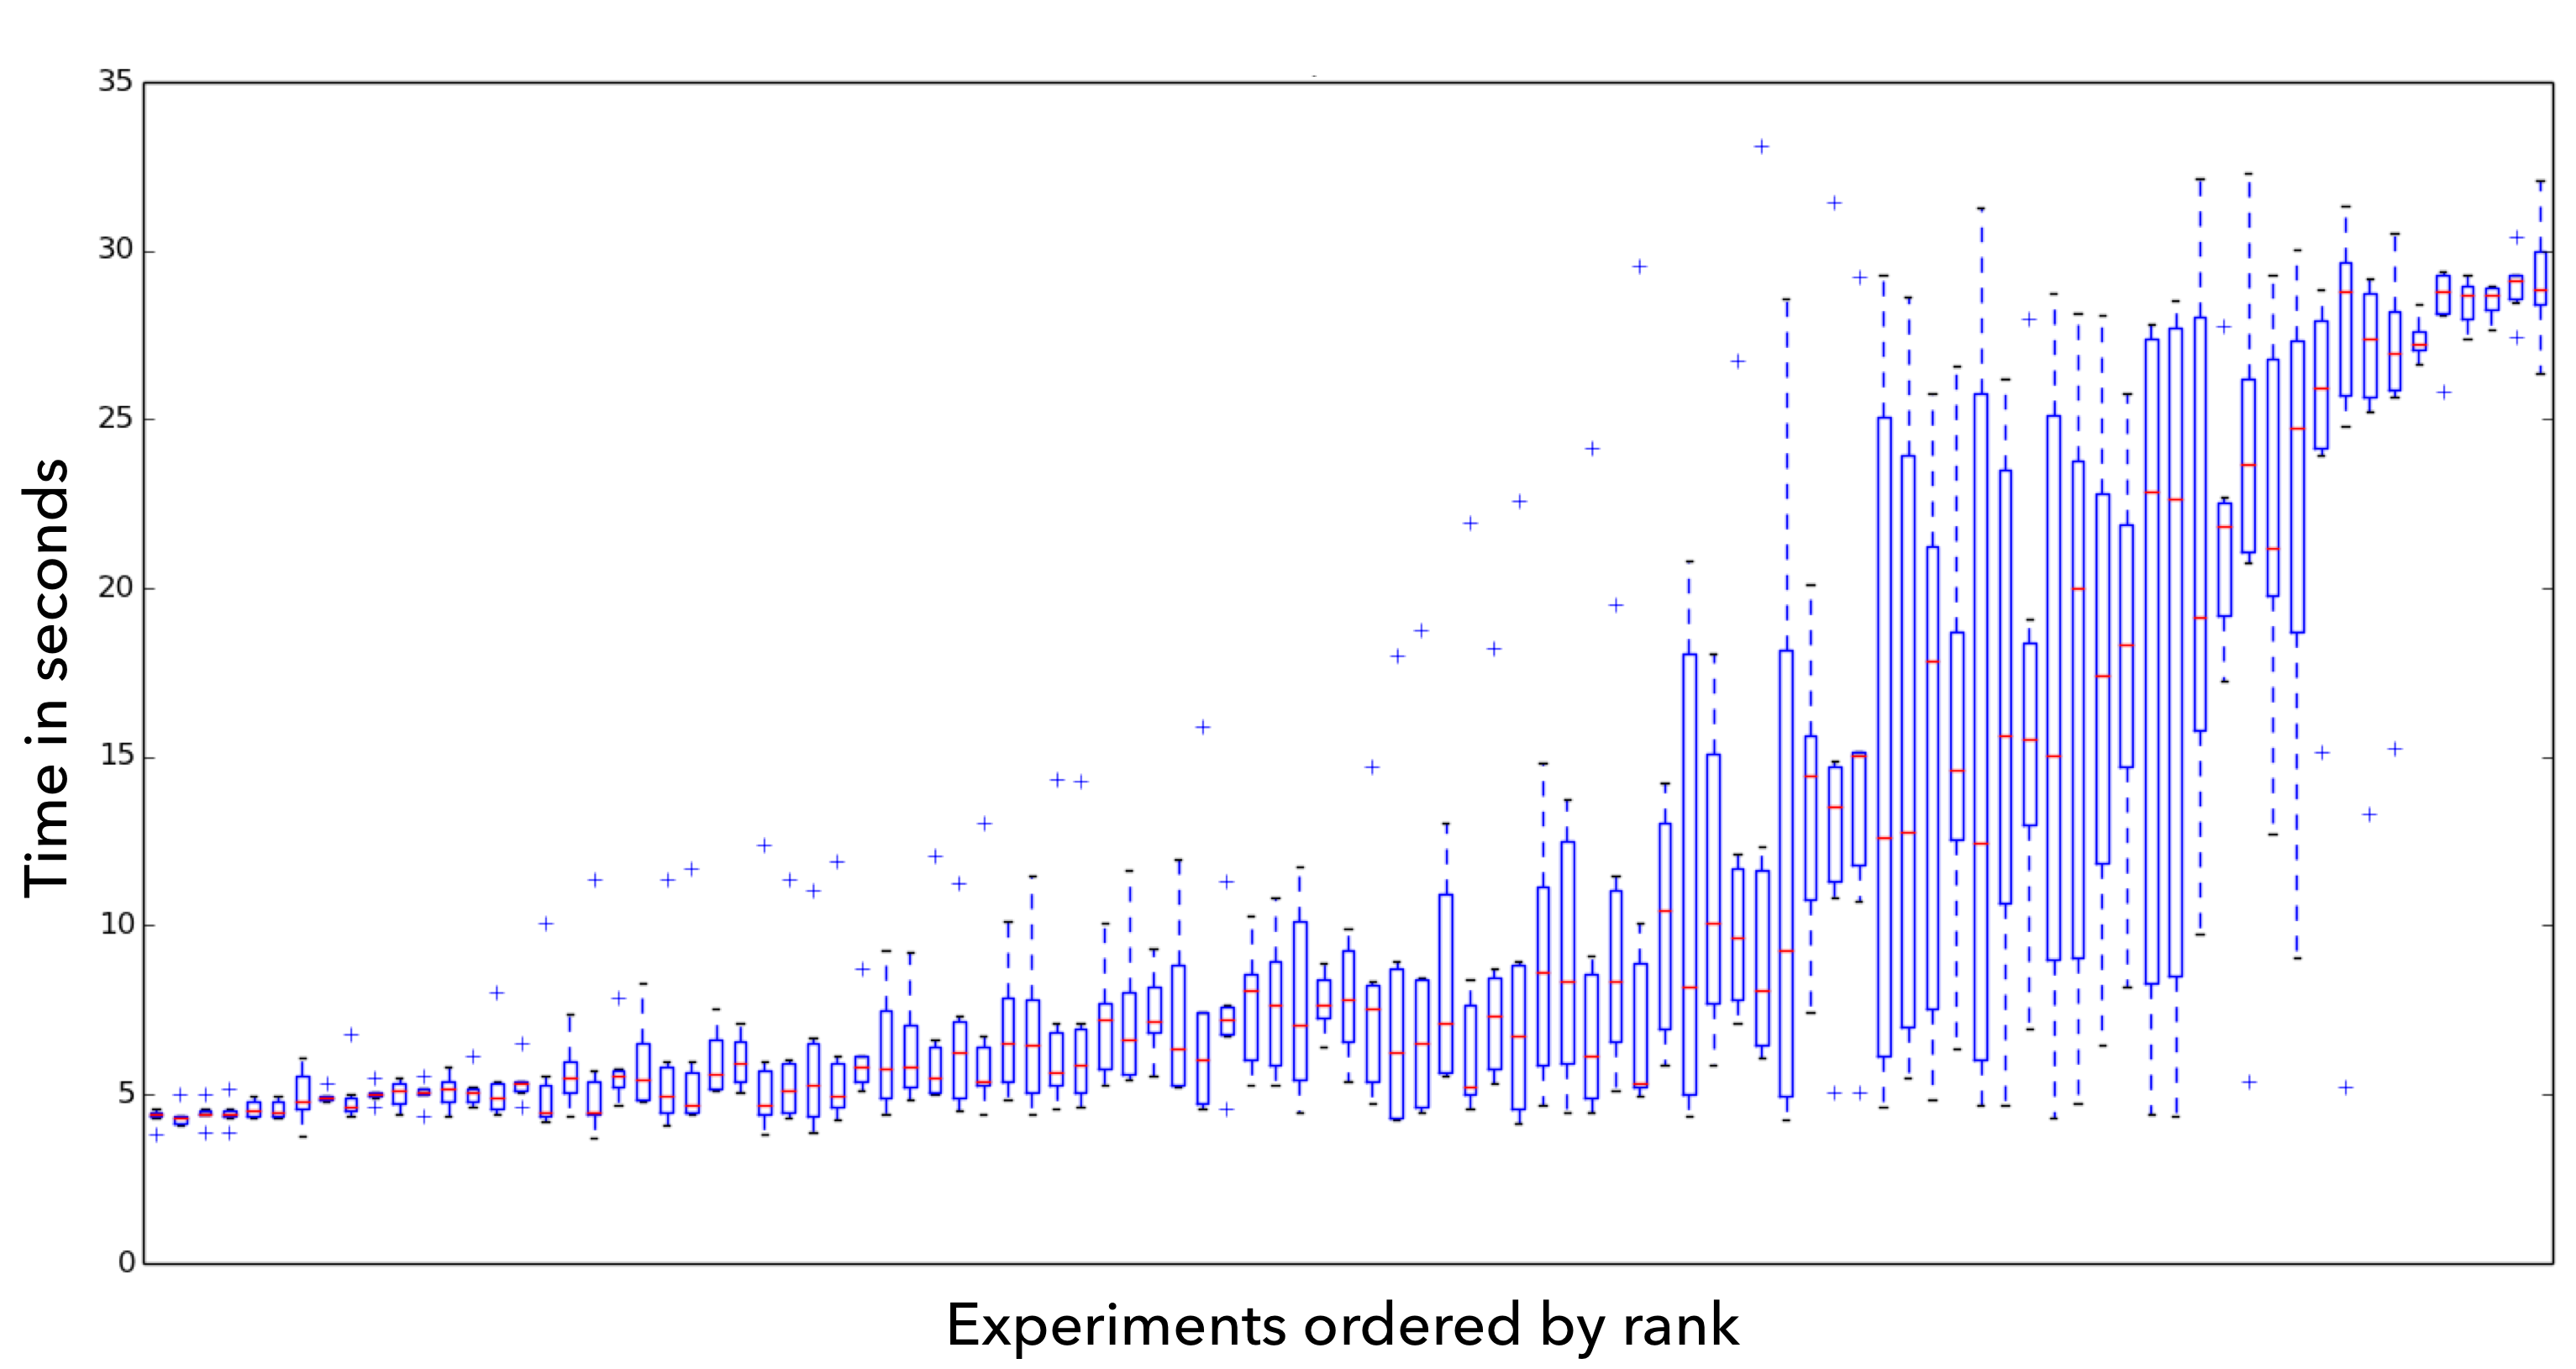
\includegraphics[width=3in]{img/6w_onemax_100_box.png}
    }
    \subfigure  [12 workers]
    {
        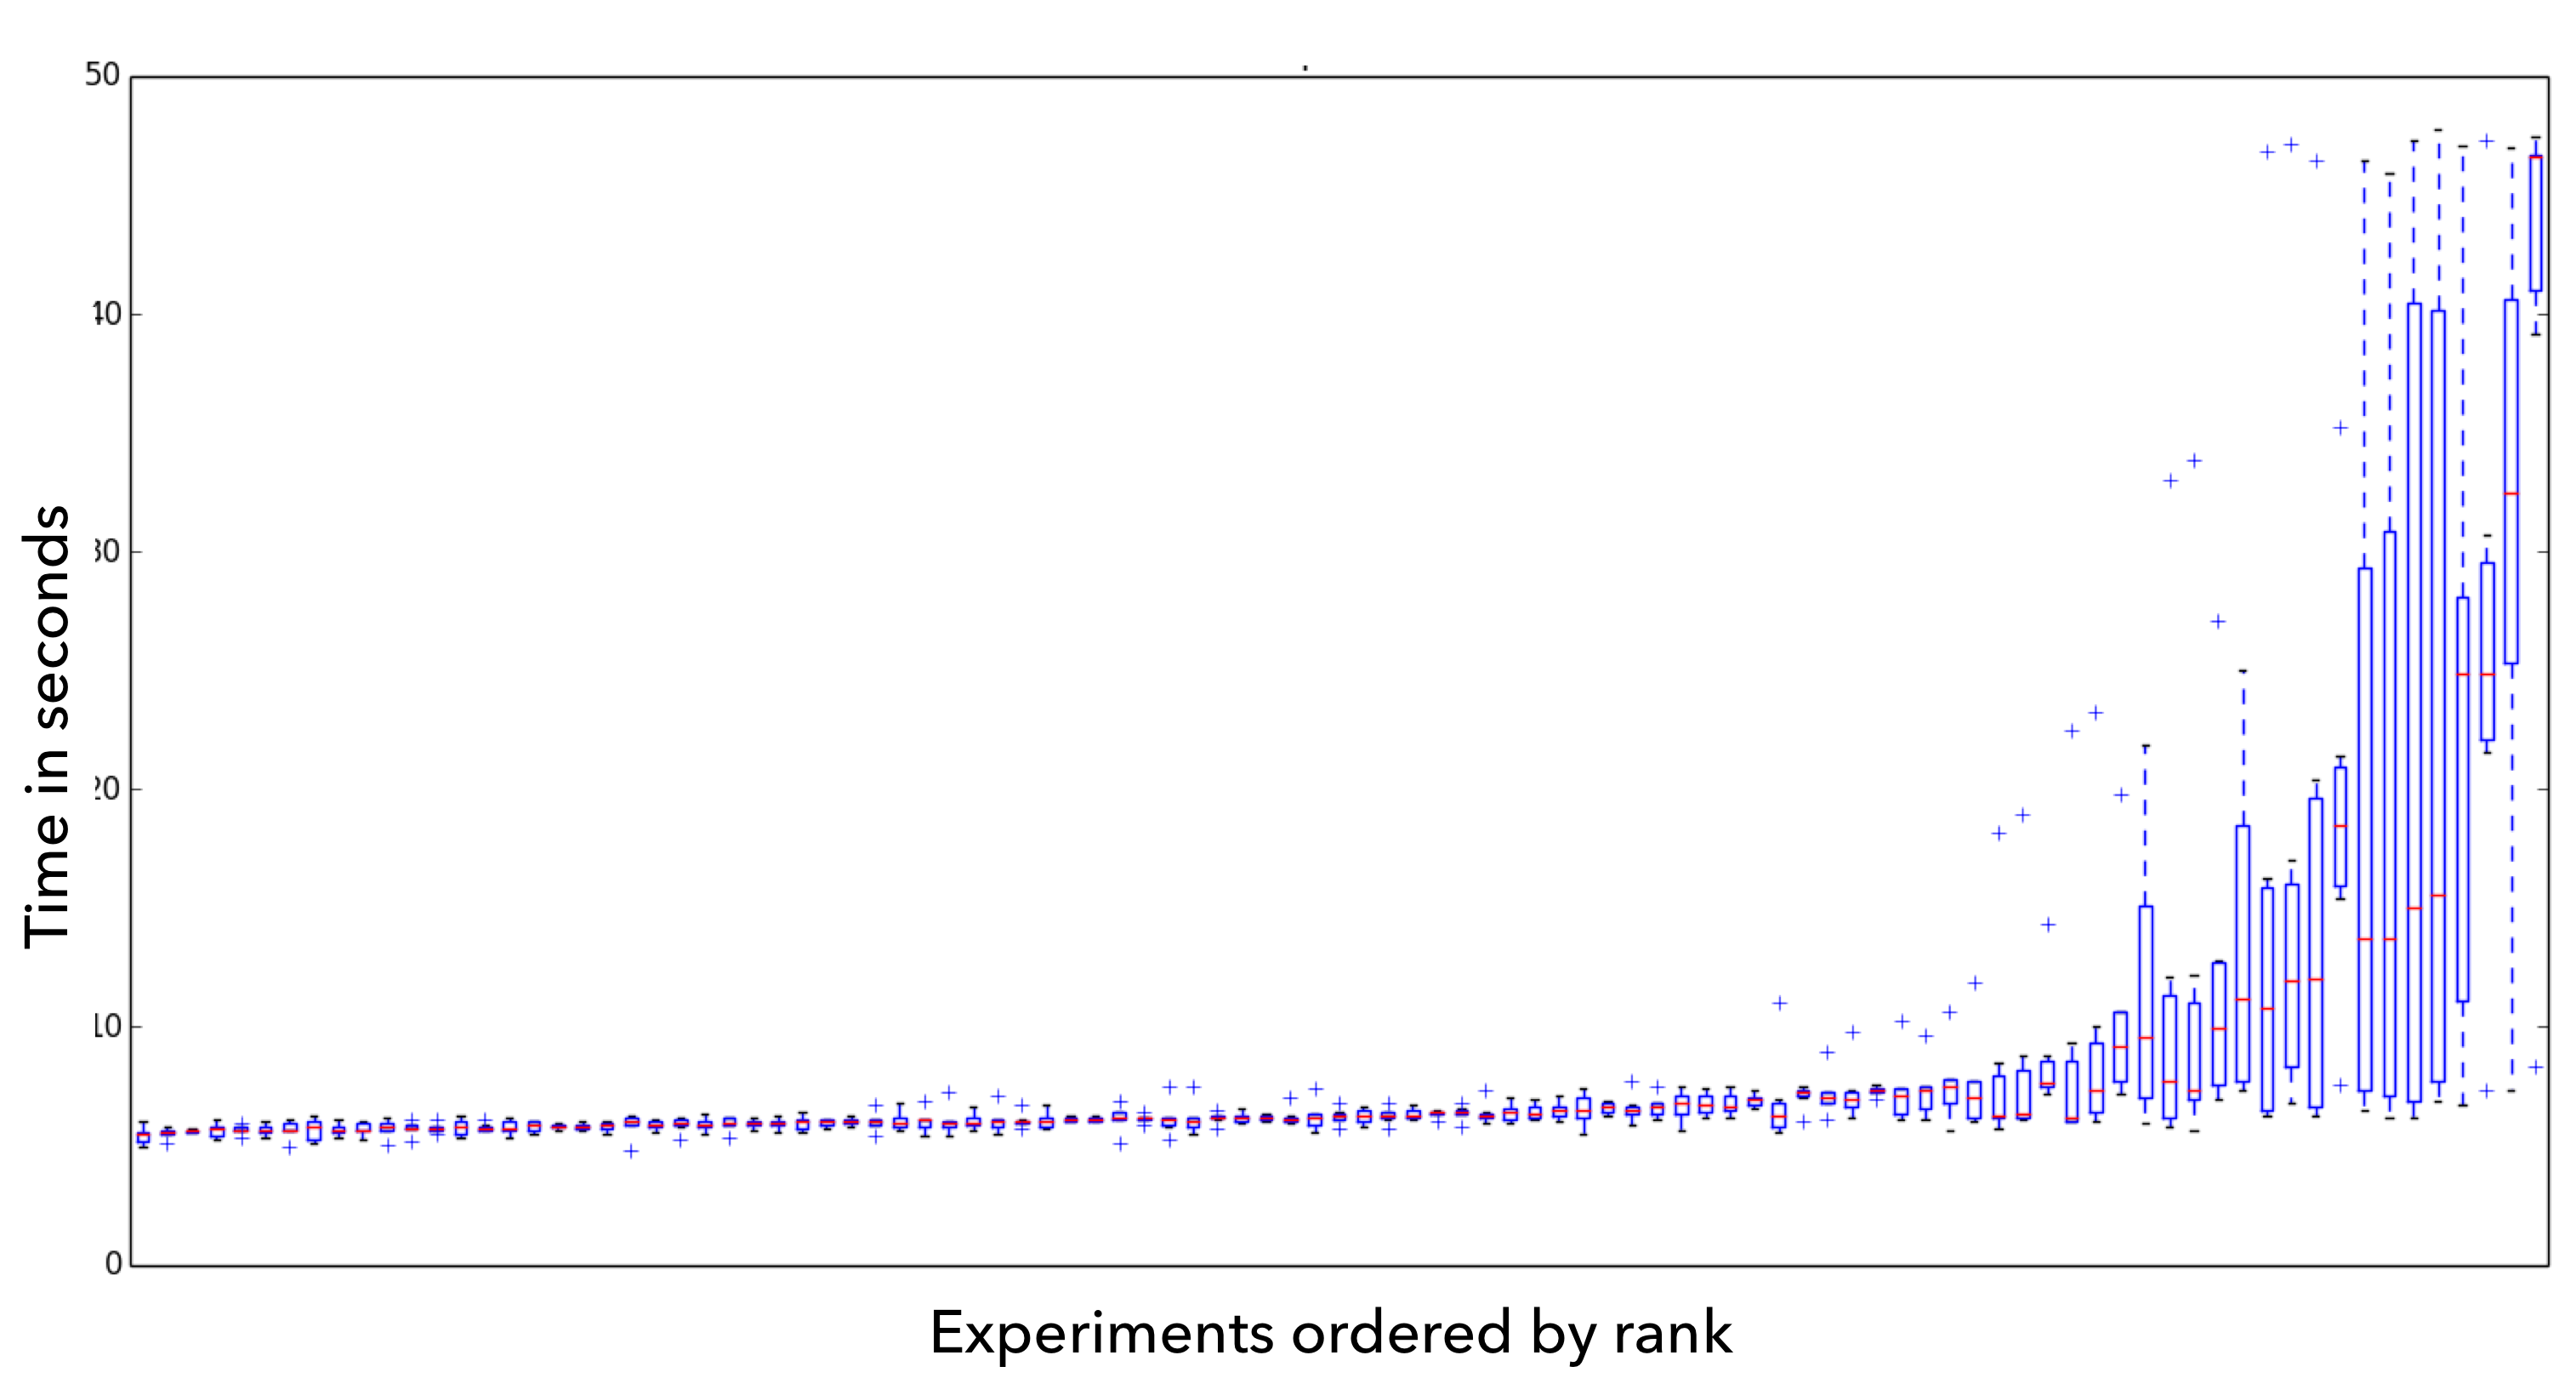
\includegraphics[width=3in]{img/12w_onemax_100_box.png}
    }

    \caption{100 experiments with random parameters for the 128 Bit OneMax problem.
    Experiments are ranked by the mean time to solution of 5 runs, with   
    (a) 2 workers, (b) 6 workers, and (c) 12 workers.}
    \label{fig:effort}
\end{figure*}


\begin{figure*}[t]
    \centering
        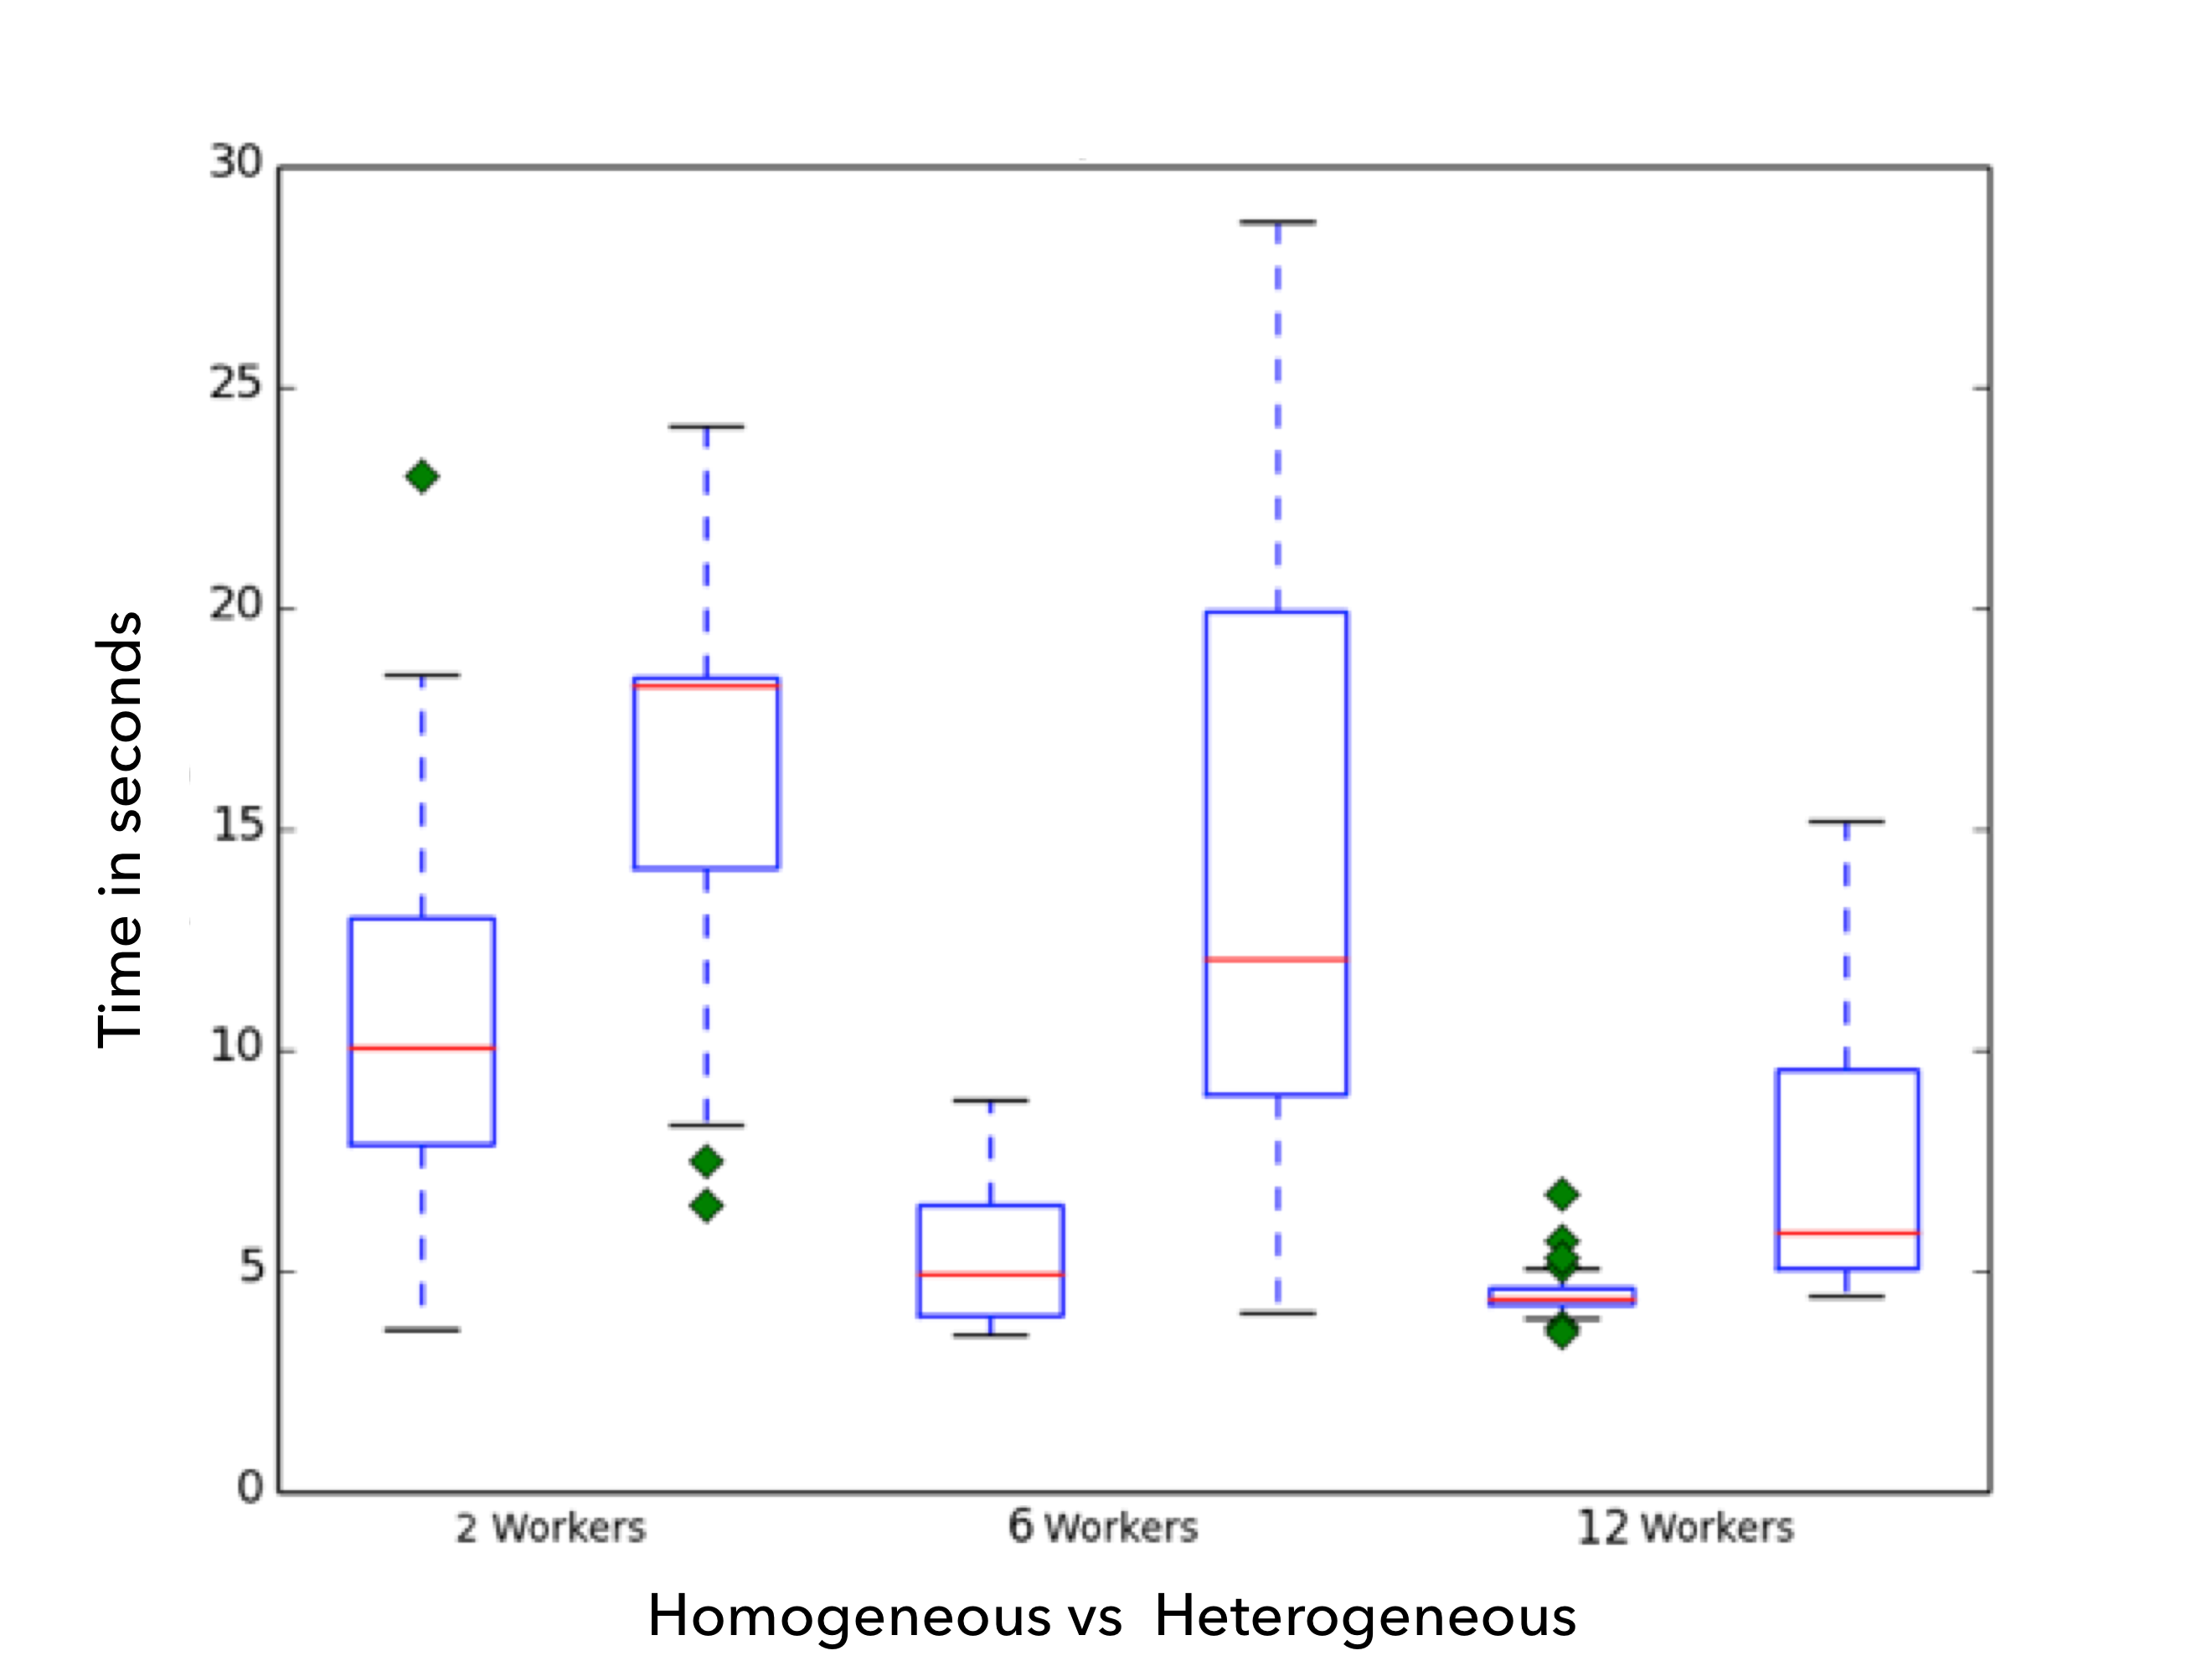
\includegraphics[width=10cm]{img/one_max_comp.png}
    \caption{Comparison of 30 runs of the 128 Bit OneMax problem. 
    Box-plot of the number of evaluations needed for solution, with a 2, 6 and 12 workers
    homogeneous configuration on the left side, and Heterogeneous configuration on the
    right side of each.
    }
    \label{fig:comp-onemax}
\end{figure*}


\subsection{ Single-Objective Optimization Test Functions}

\begin{figure*}[b]
    \centering
    \subfigure  [6 workers]
    {
        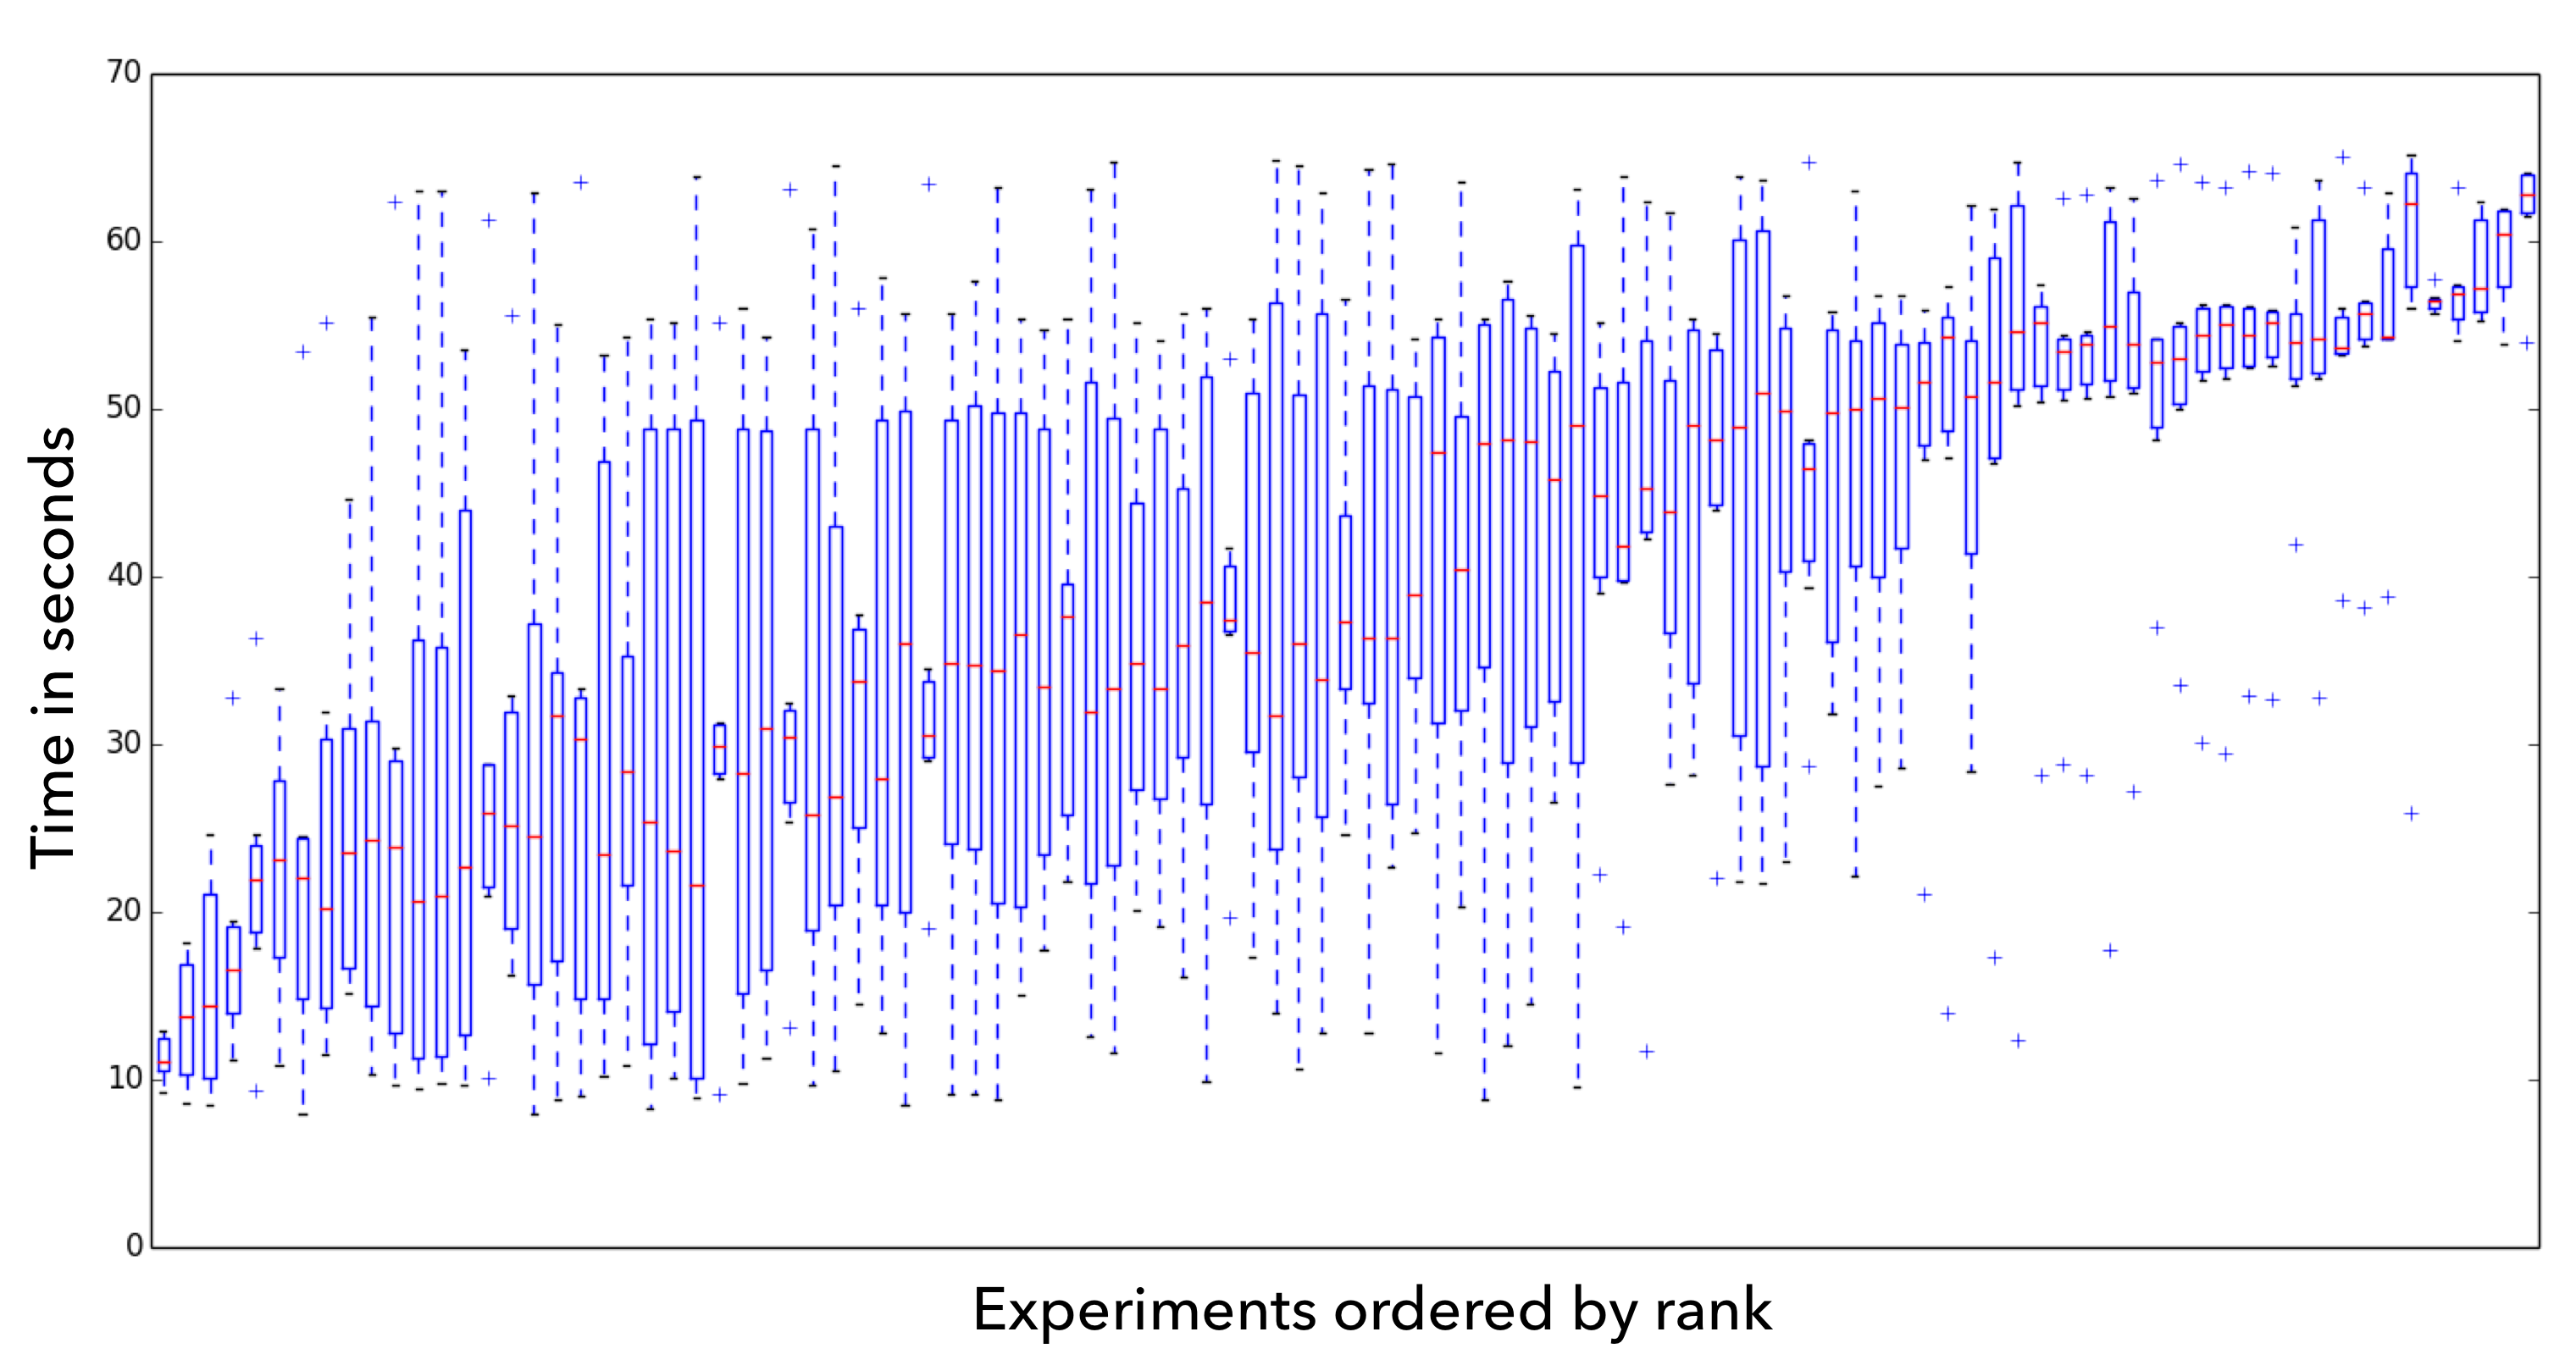
\includegraphics[width=2.2in]{img/6w_griewank_100_box.png}
    }
    \subfigure  [12 workers]
    {
        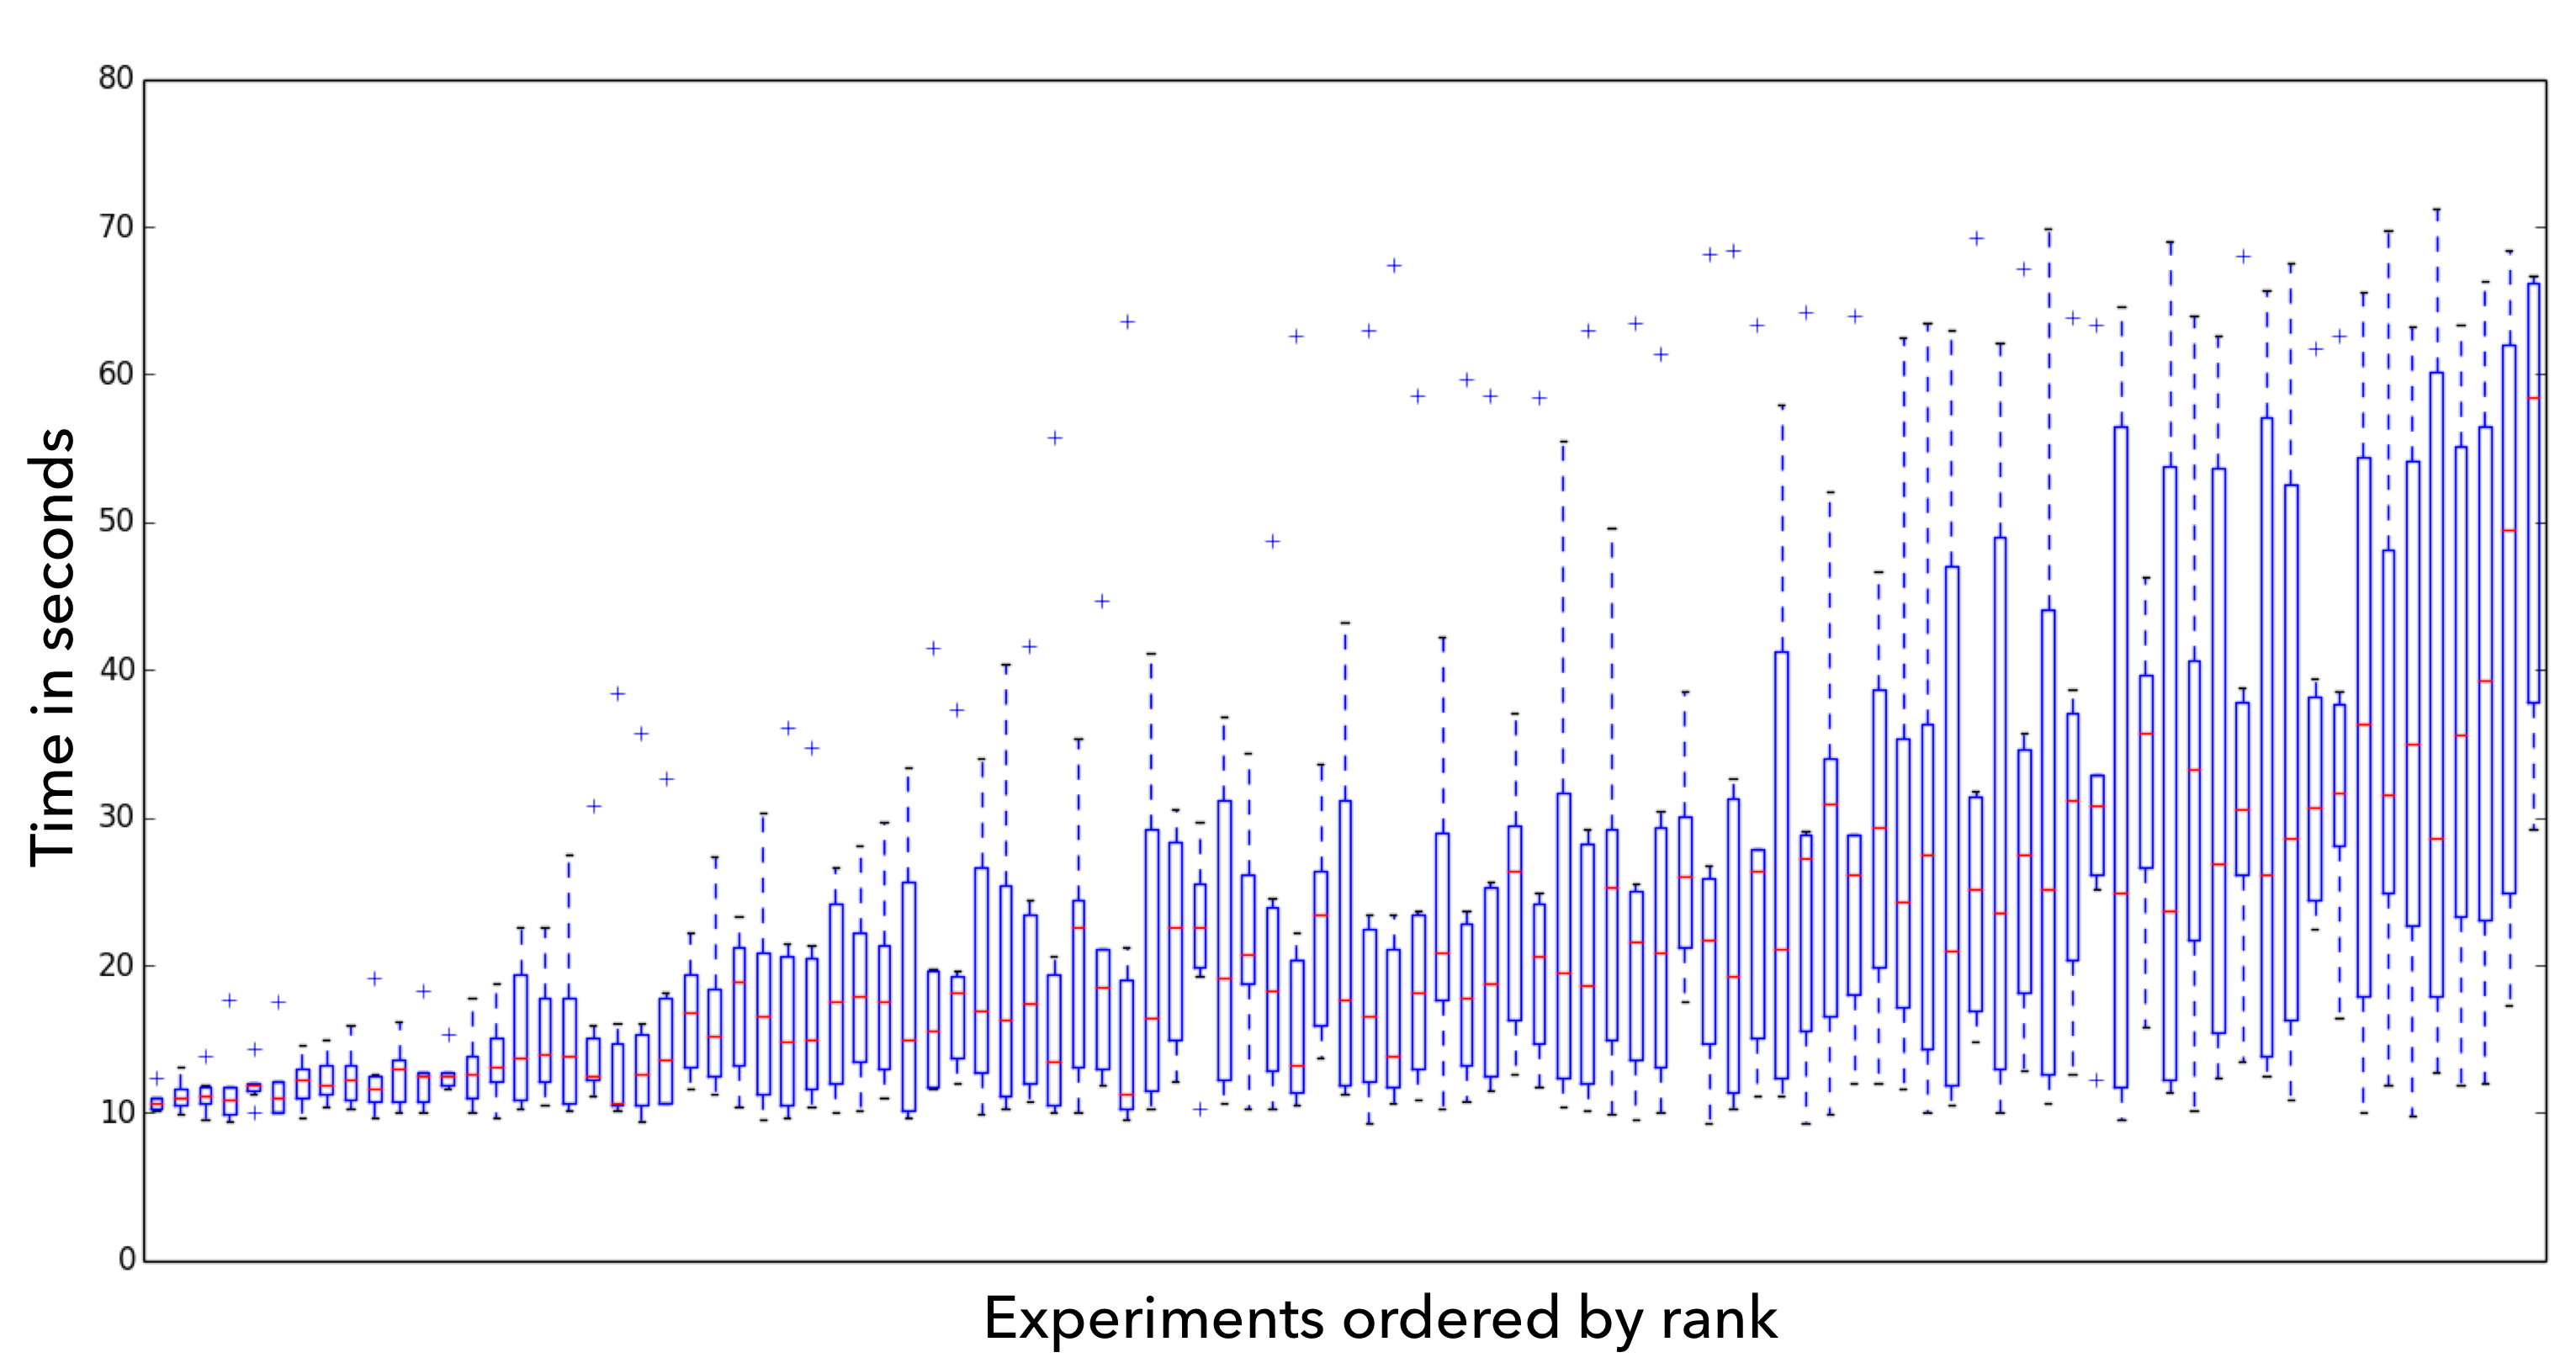
\includegraphics[width=2.2in]{img/12w_griewank_100_box.png}
    }

    \caption{100 experiments with random parameters for the 128 Bit Griewank 
    single-objective optimization test function. Experiments are ranked by 
    the mean time to solution of 5 runs, with (a) 6 workers, and (b) 12 workers.}
    \label{fig:griewank-homo}
\end{figure*}


\begin{figure*}[b]
    \centering
    \subfigure  [Homogeneous]
    {
        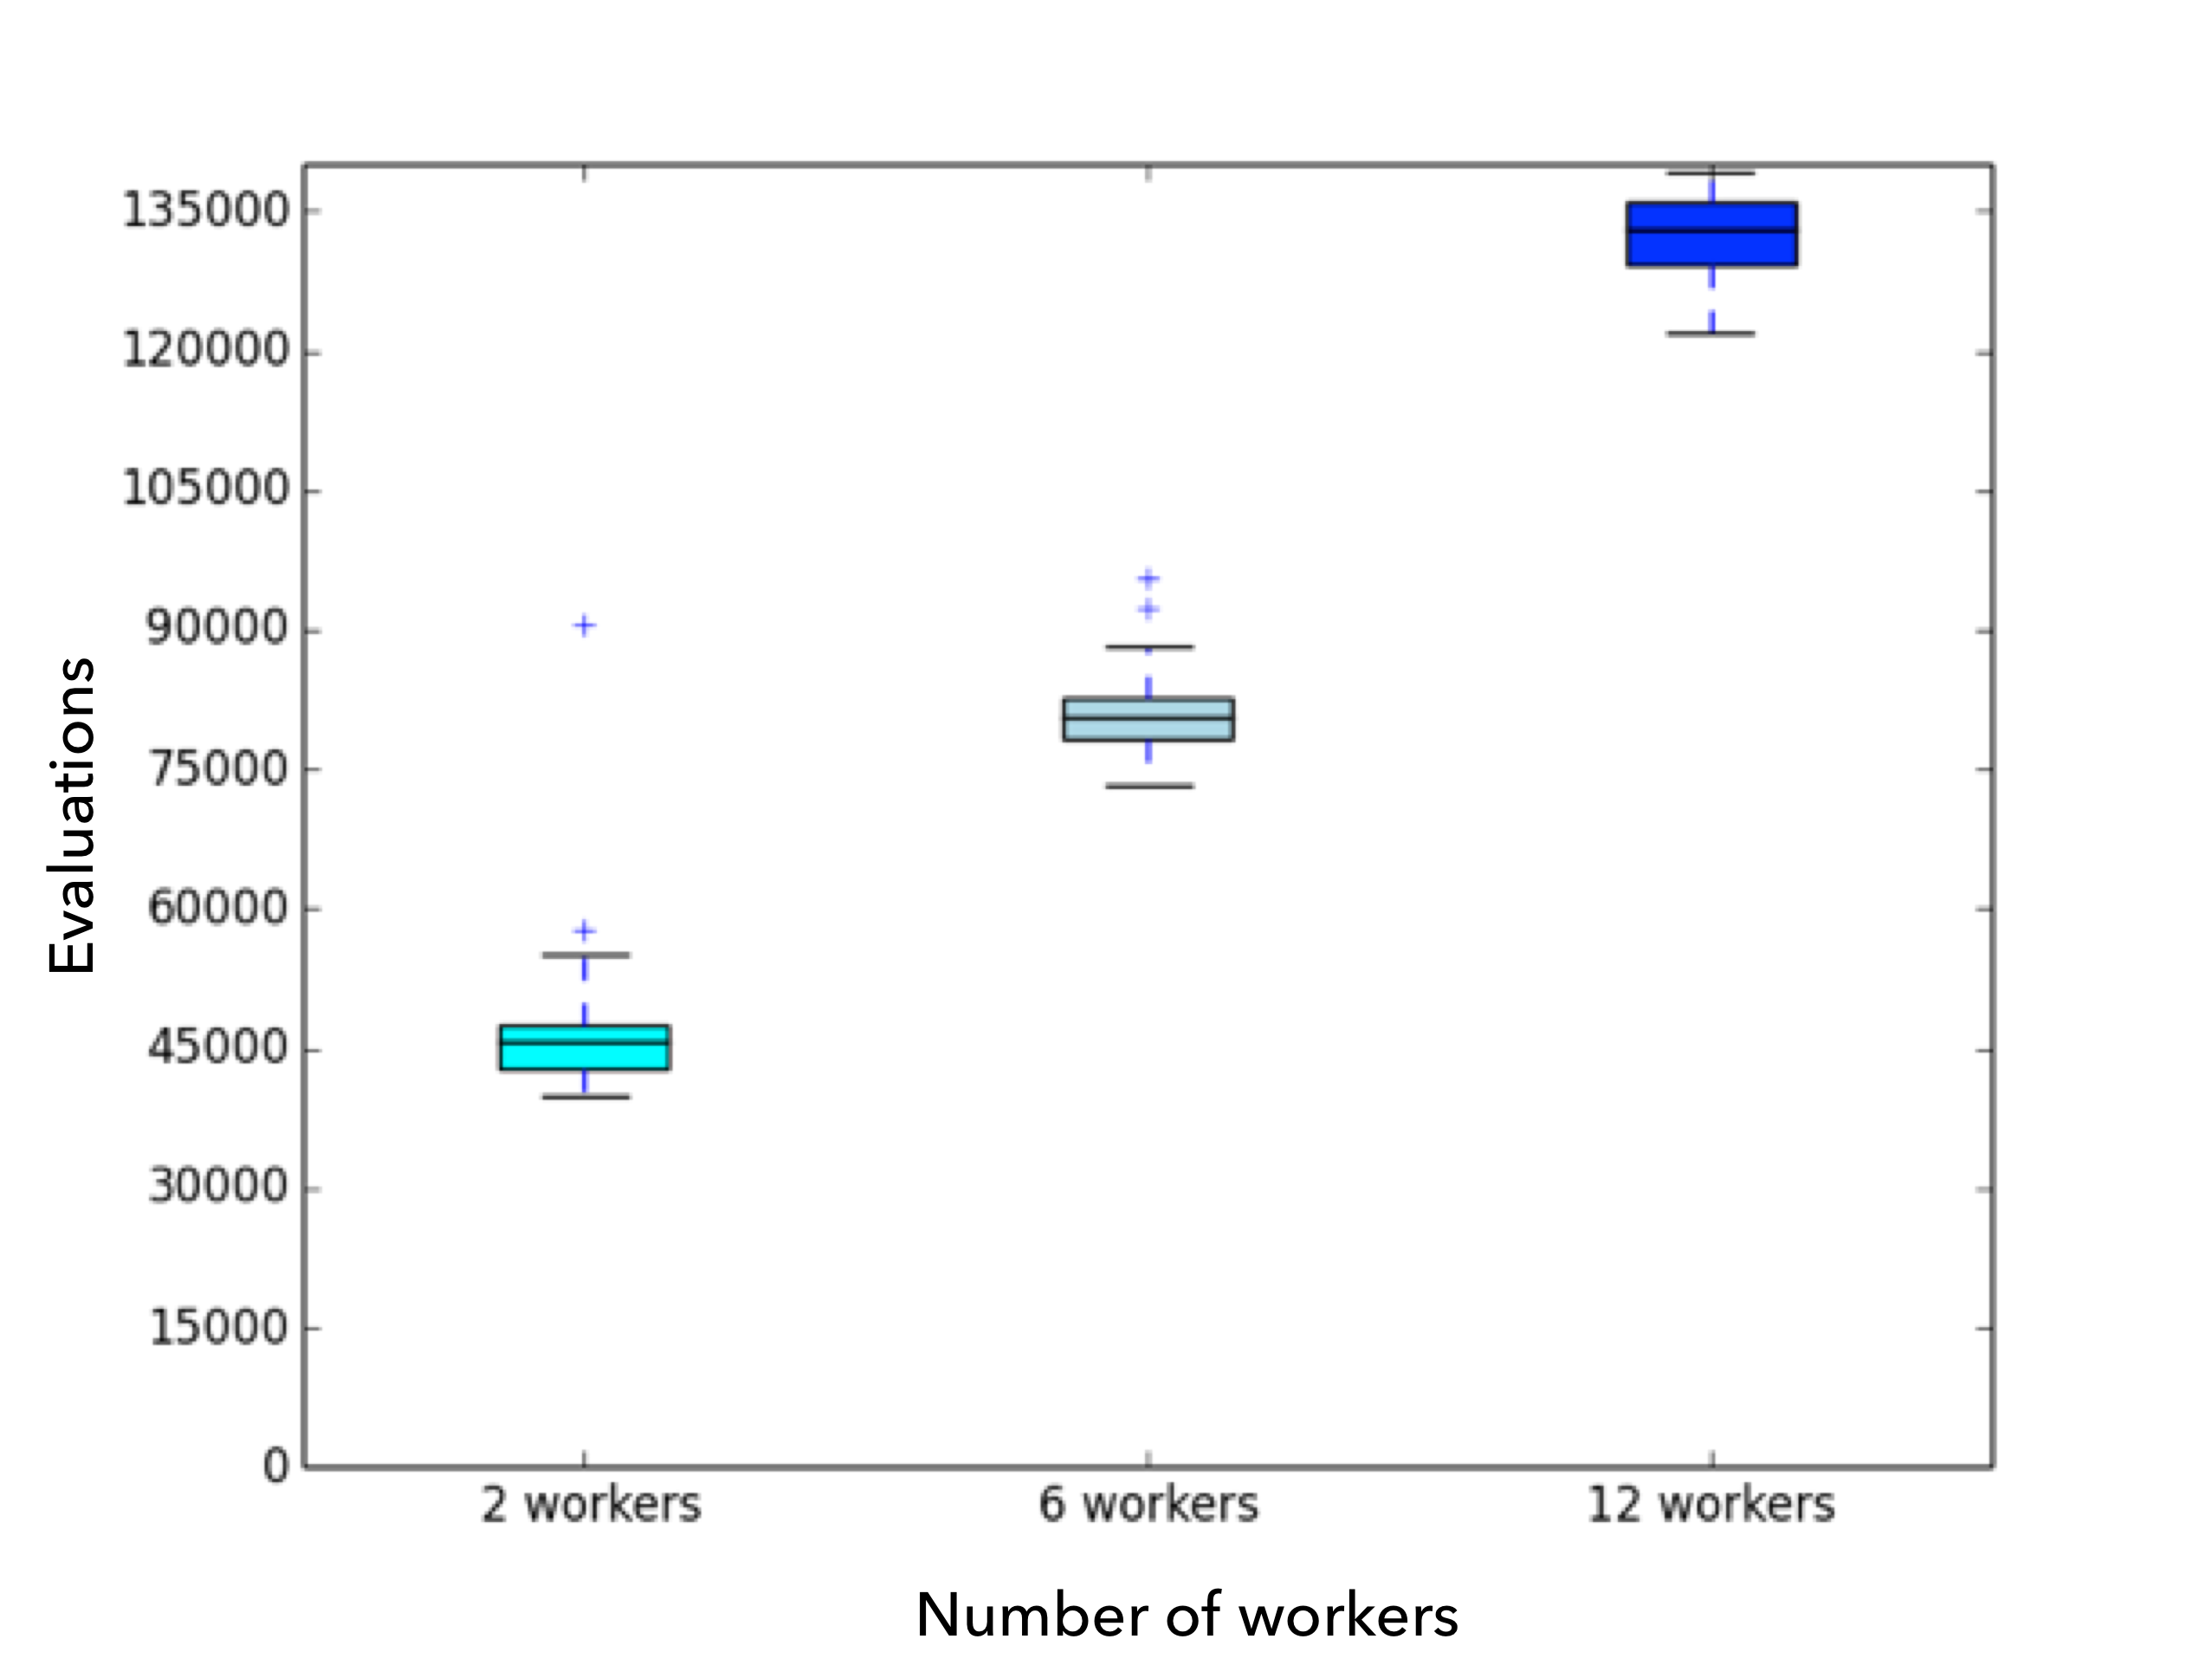
\includegraphics[width=2.2in]{img/griewank_evals_homo.png}
    }
    \subfigure  [Heterogeneous]
    {
        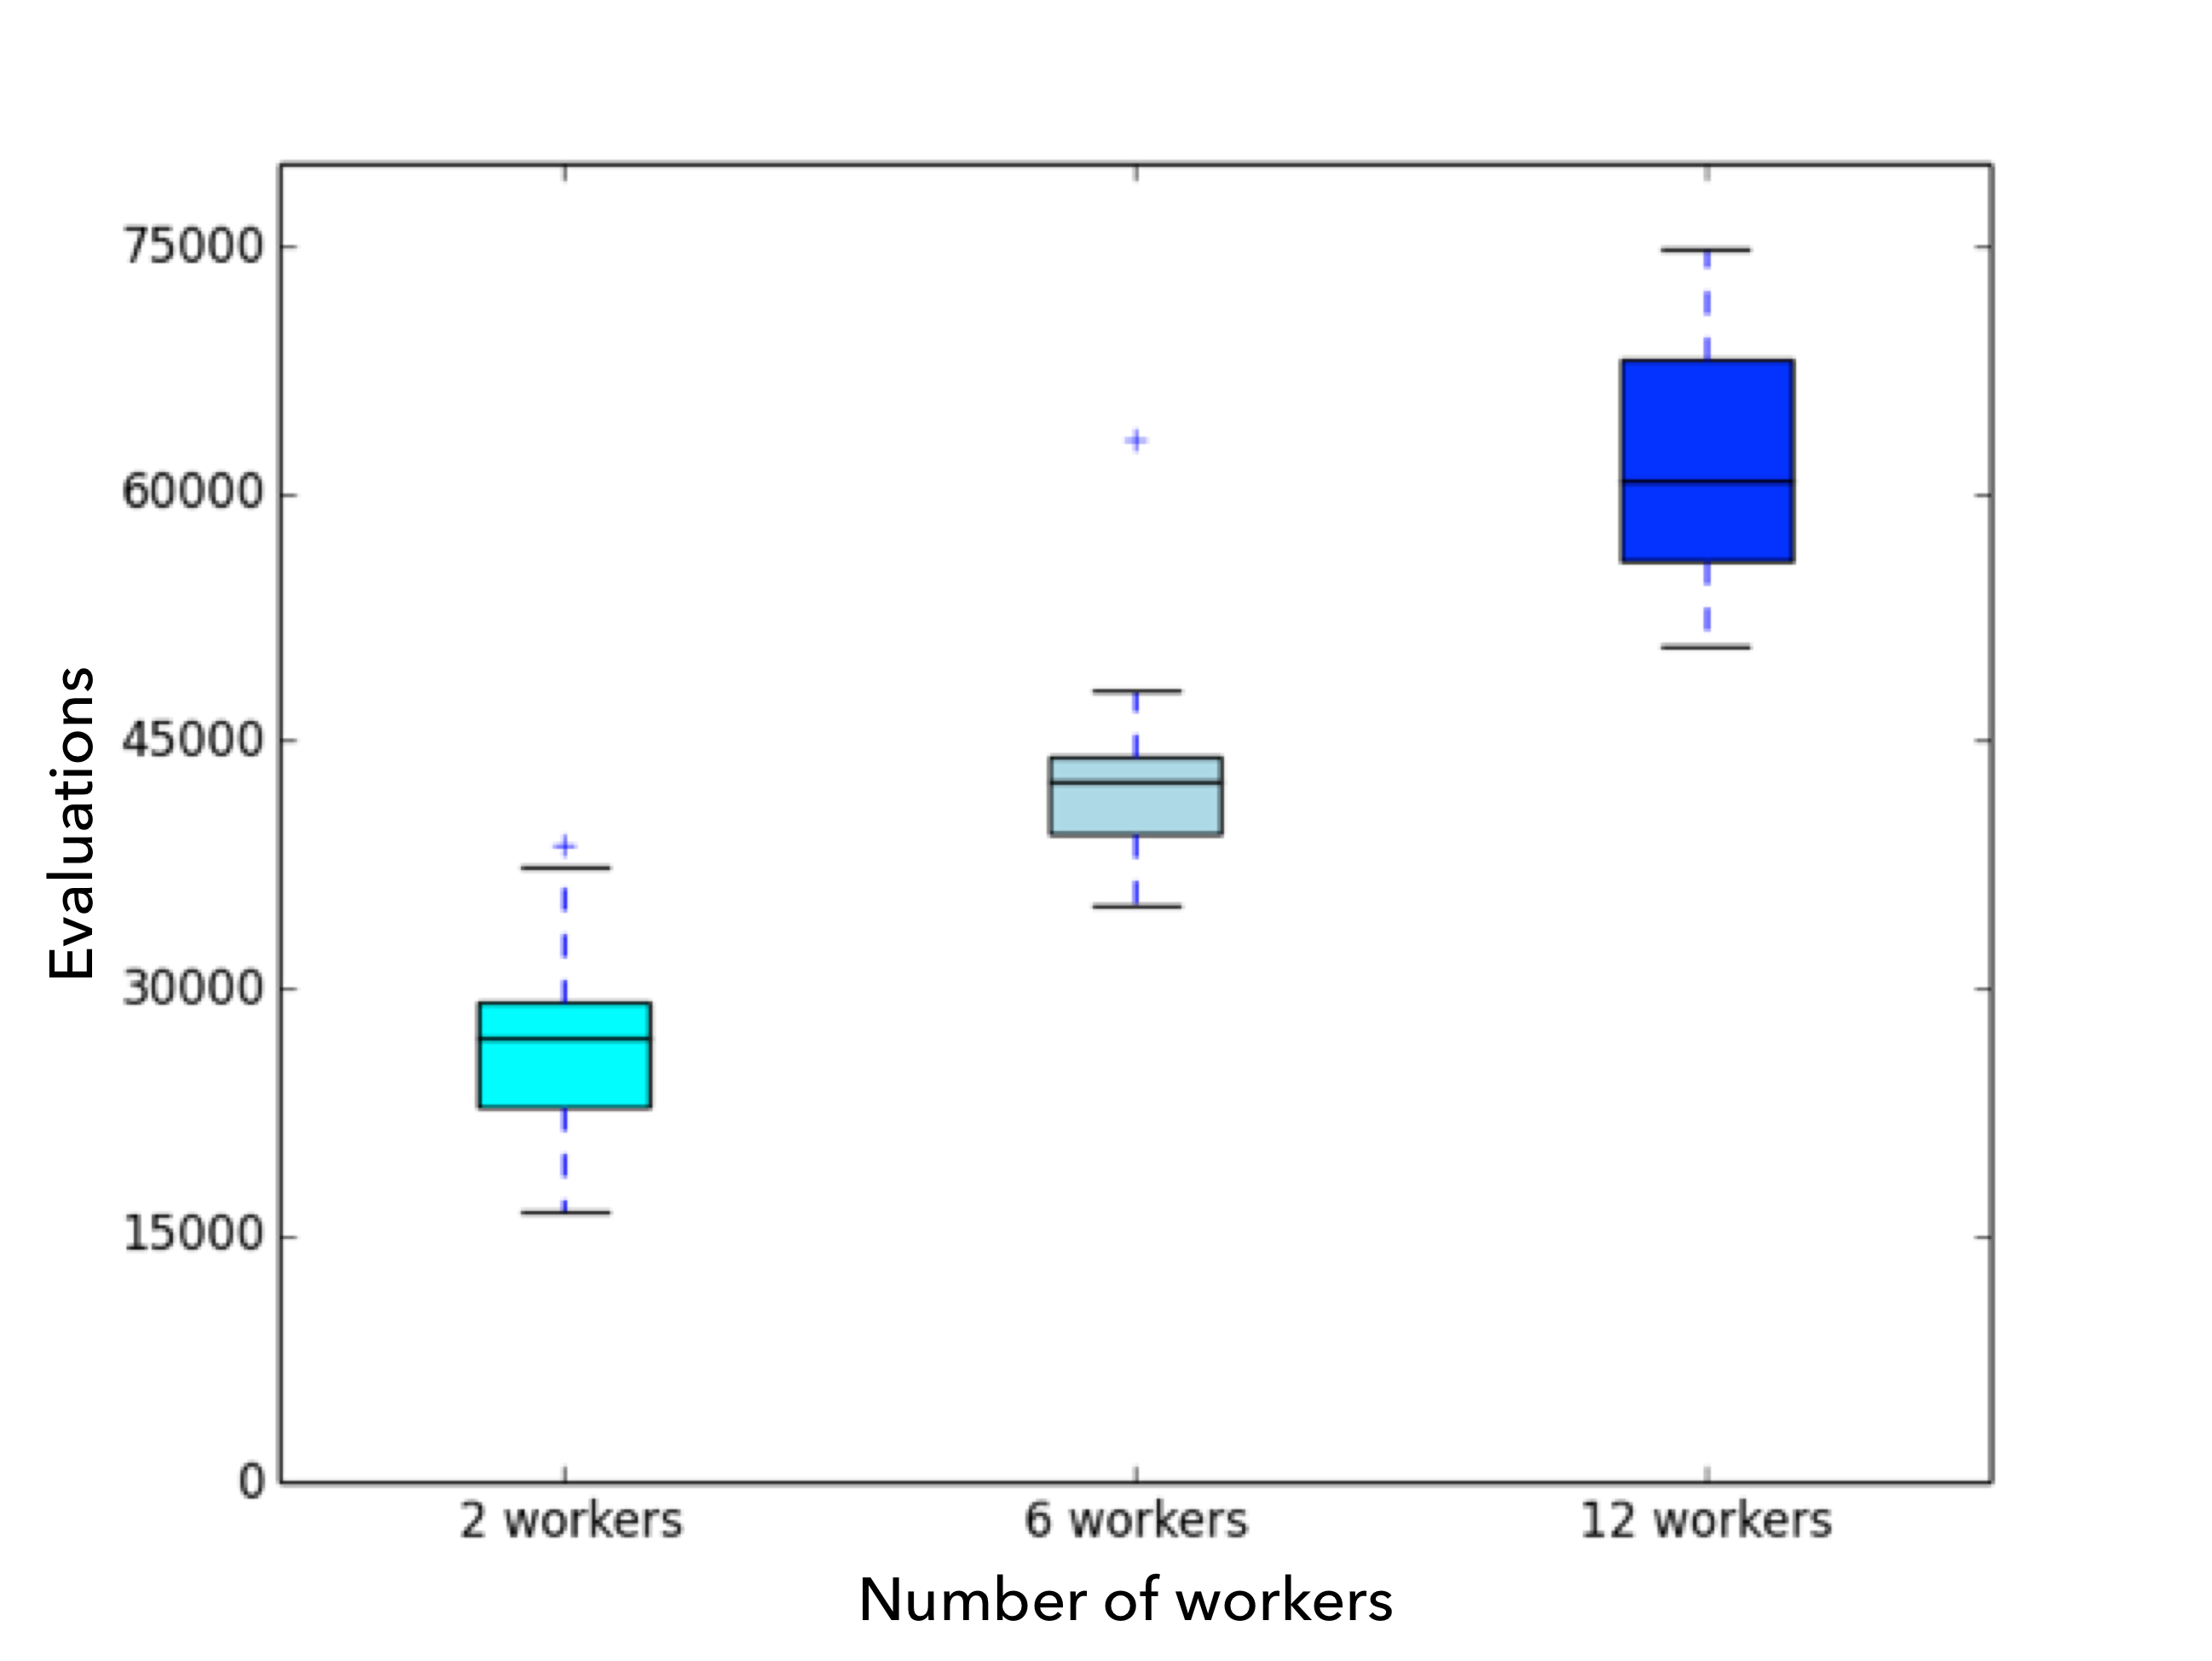
\includegraphics[width=2.2in]{img/griewank_evals_hetereo.png}
    }
      \caption{30 runs of the 128 dimension Griewank single-objective optimization test function. 
    Box-plot of the number of evaluations needed for solution, with an (a) Homogeneous configuration, and (b) Heterogeneous configuration.}
    \label{fig:griewank-evals}
\end{figure*}

\begin{figure*}[b]
    \centering
    \subfigure  [Homogeneous]
    {
        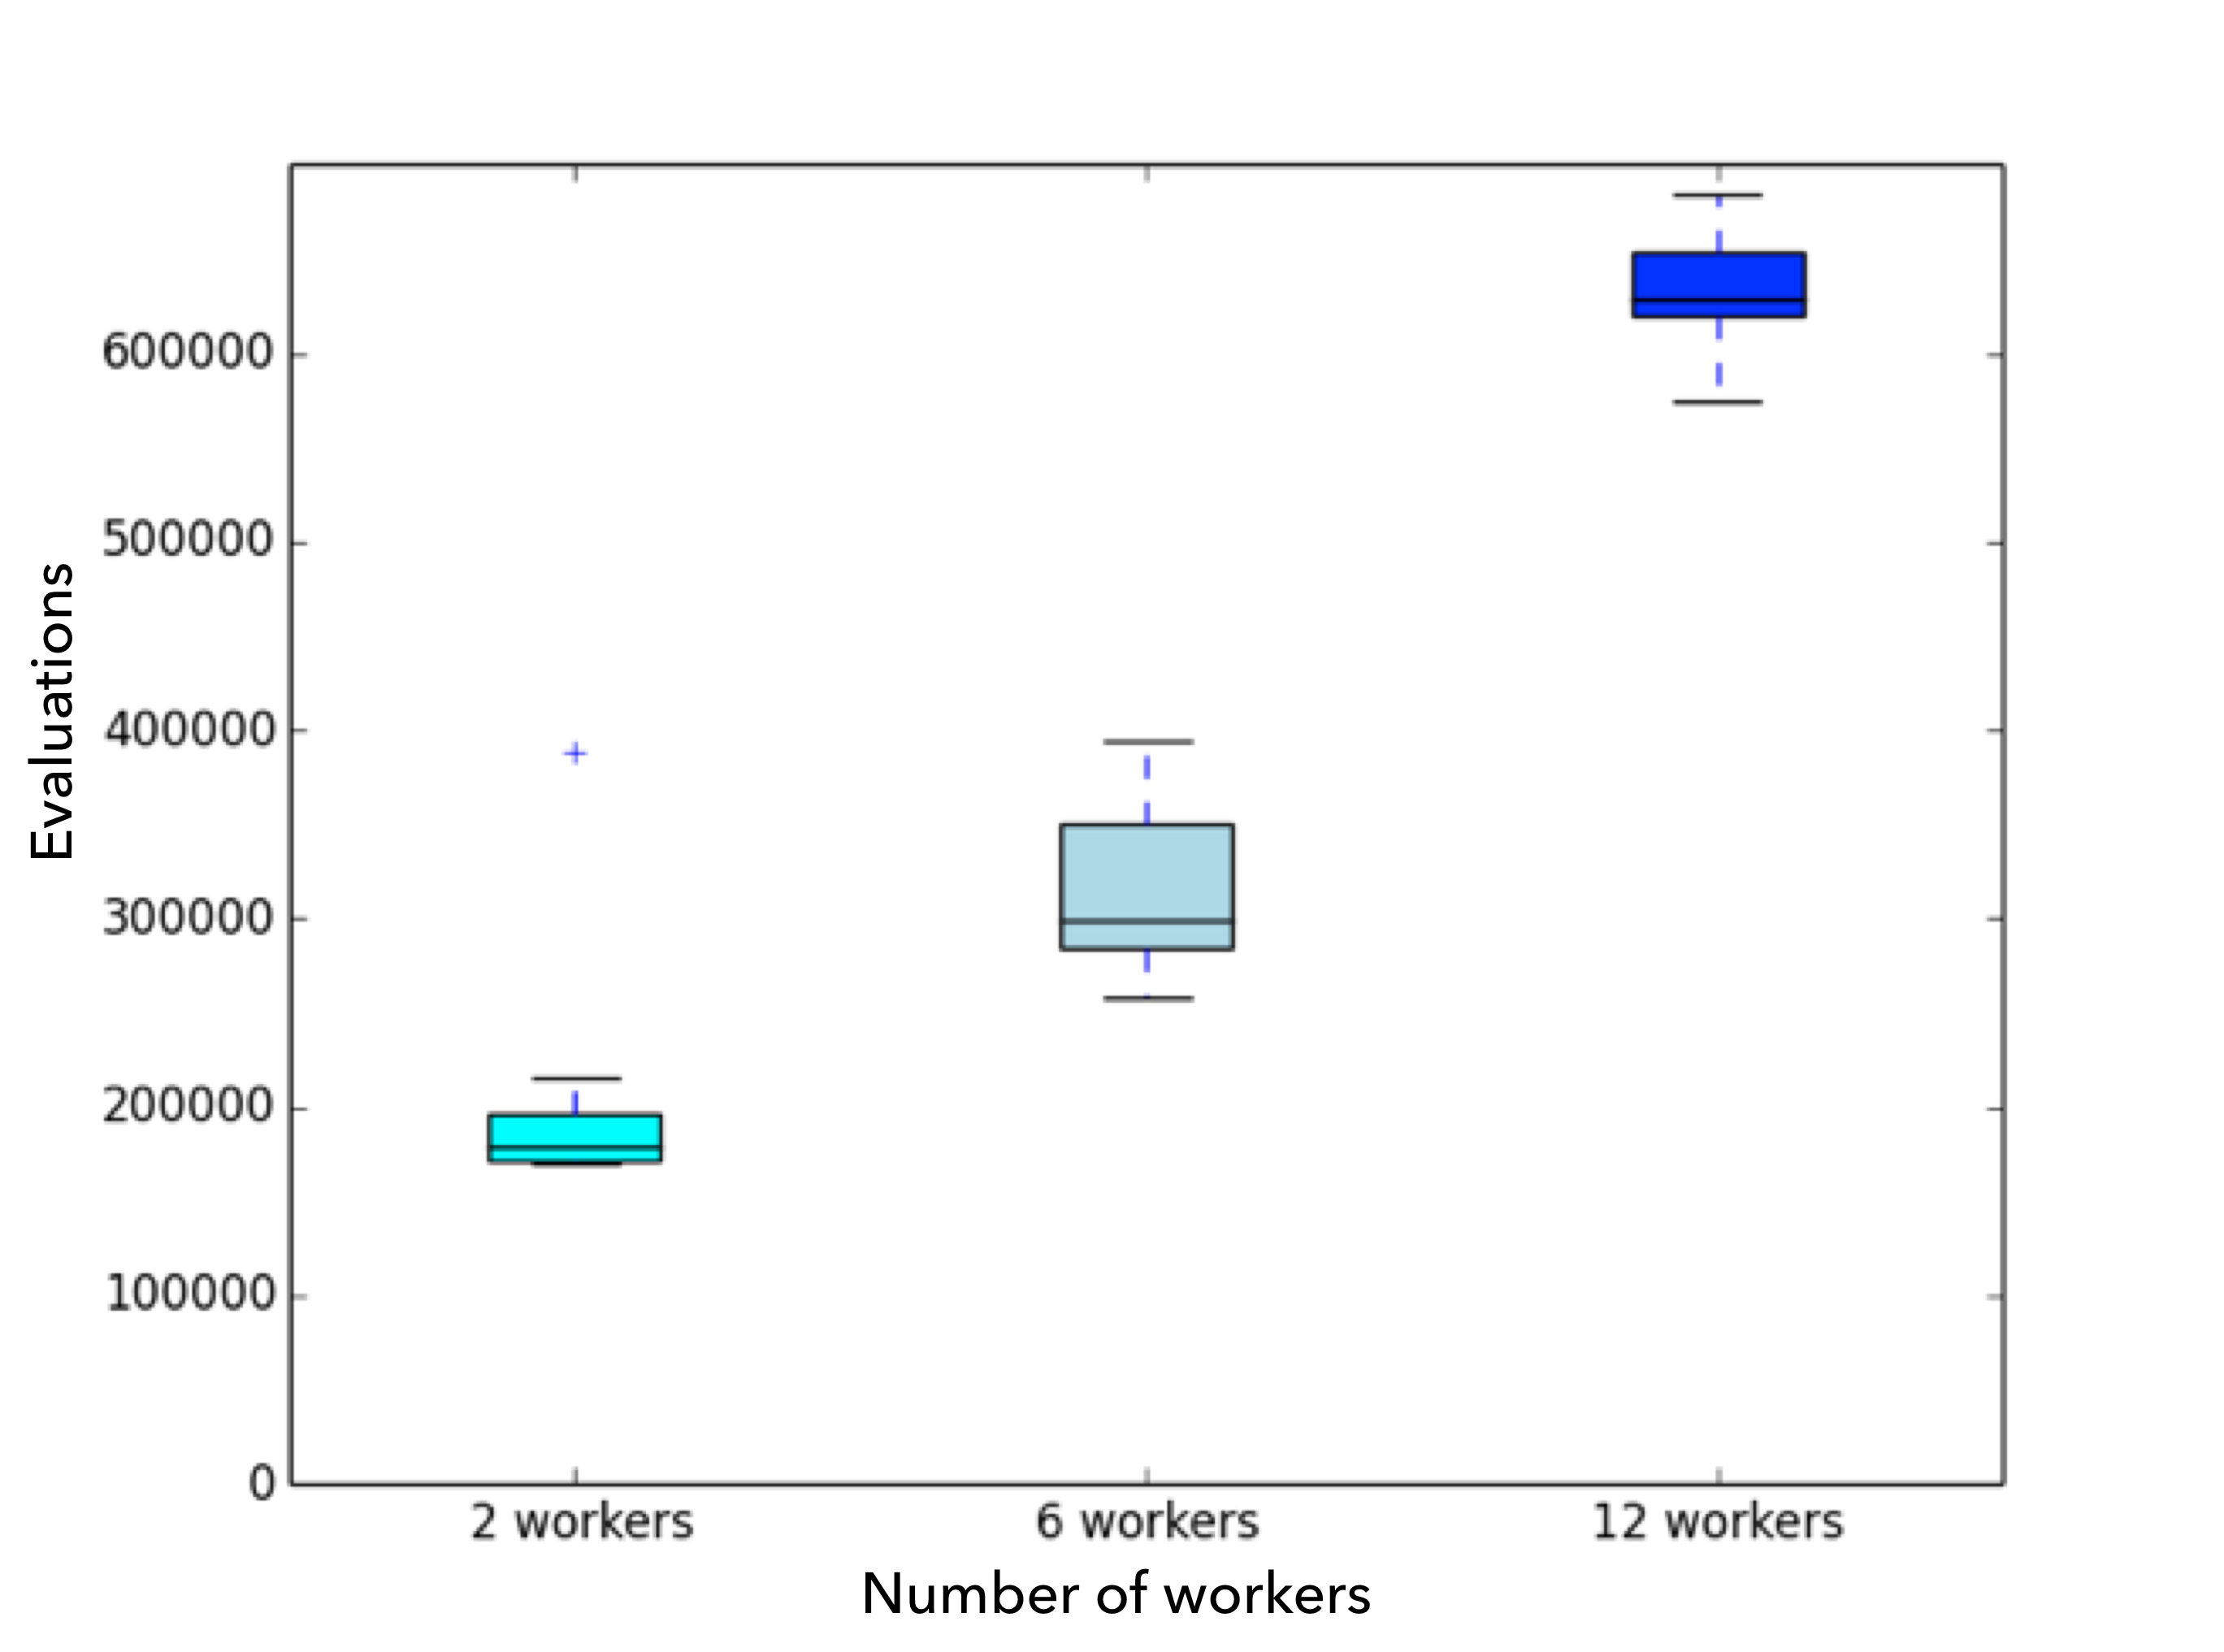
\includegraphics[width=2.2in]{img/schaffer_evals_homo.png}
    }
    \subfigure  [Heterogeneous]
    {
        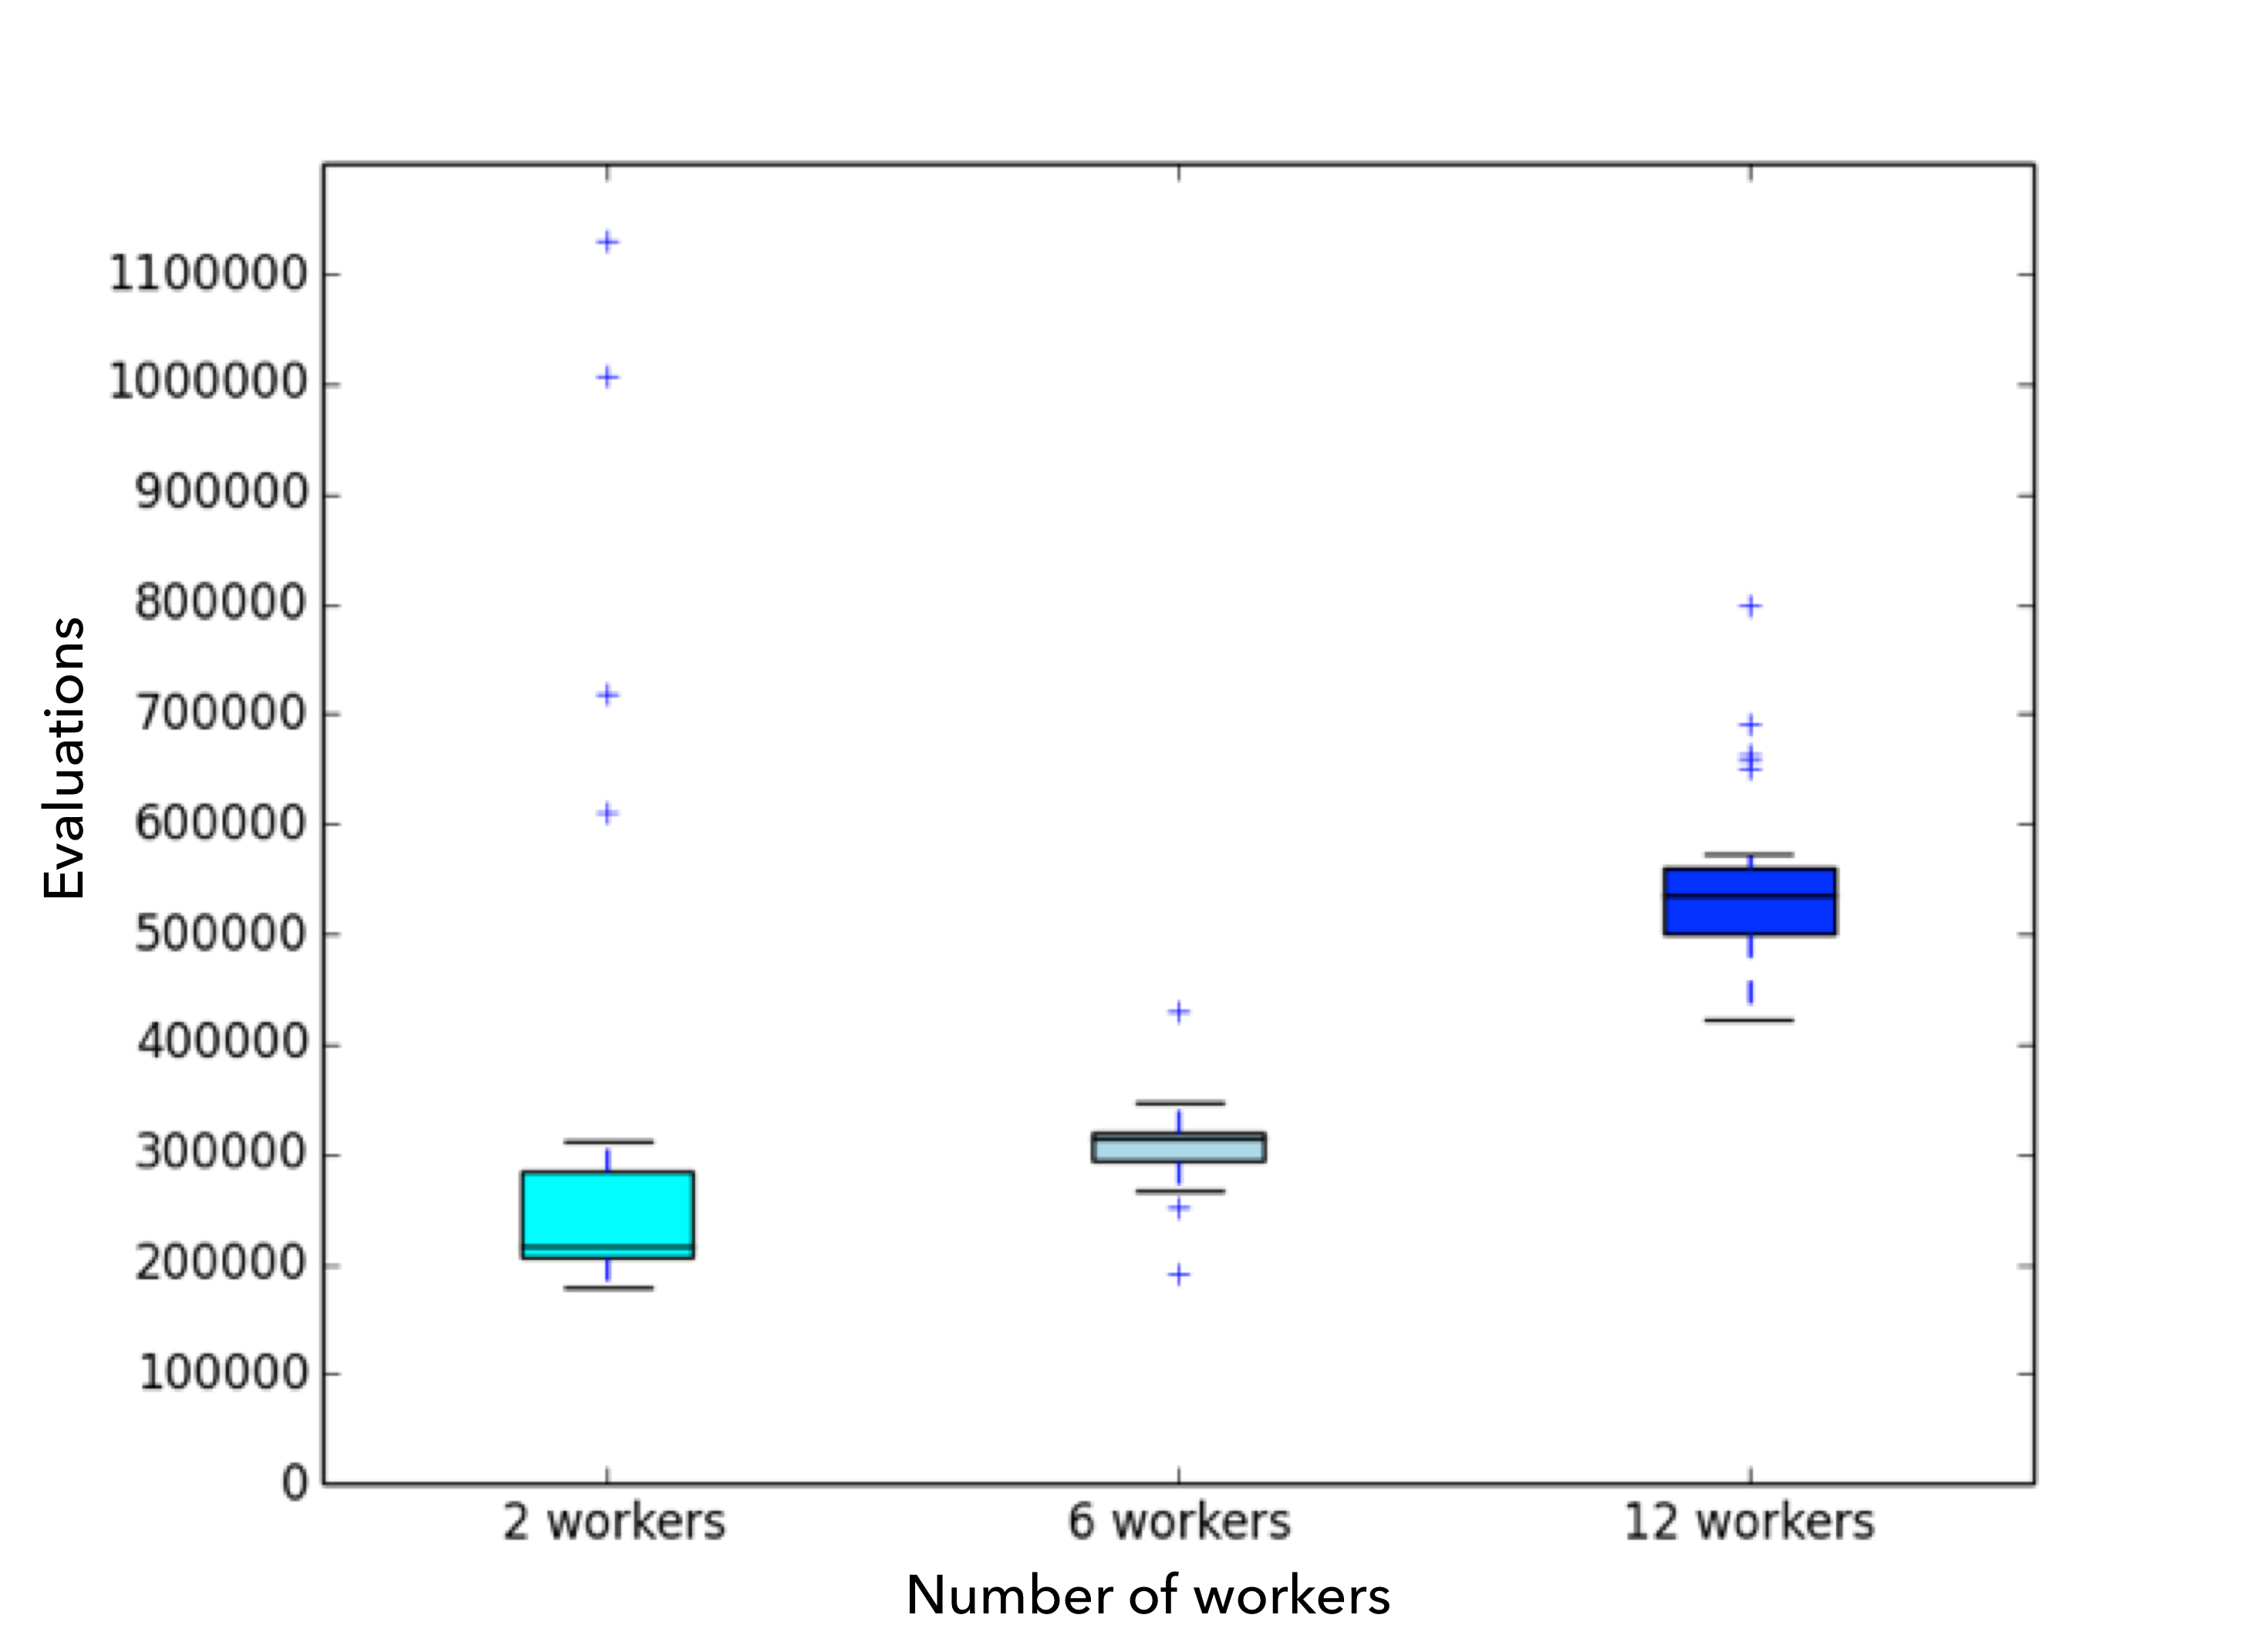
\includegraphics[width=2.2in]{img/schaffer_evals_hetereo.png}
    }
 

    \caption{30 runs of the 128 dimension Schaffer single-objective optimization test function. 
    Box-plot of the number of evaluations needed for solution, with an (a) Homogeneous configuration, and (b) Heterogeneous configuration.}
    \label{fig:schaffer-evals}
\end{figure*}

\begin{figure*}[t]
    \centering
        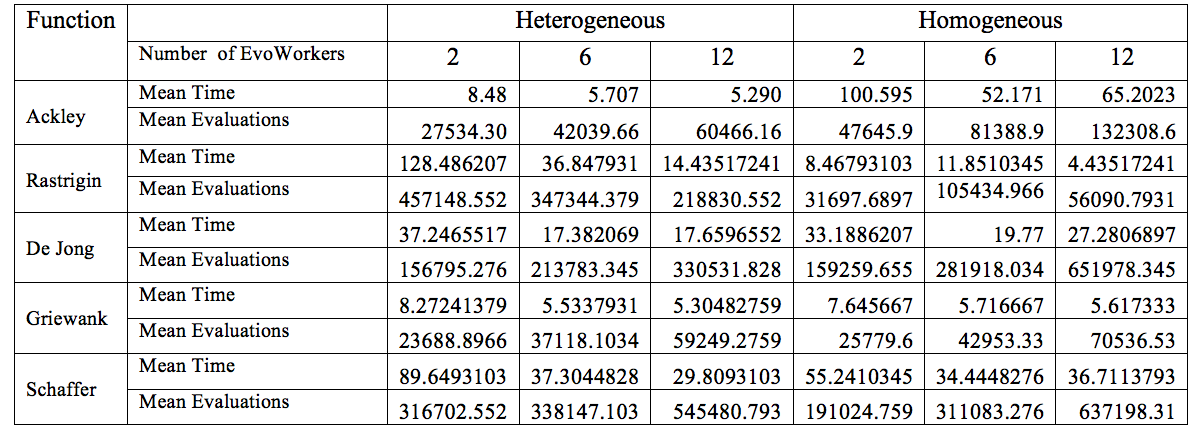
\includegraphics[width=10cm]{img/table.png}
    \caption{Summary table of results. }
    \label{fig:summary}
\end{figure*}

\end{document}
